
%%%%%%%%%%%%%%%
% START COPY %%
%%%%%%%%%%%%%%%

\epigraph{\singlespacing ``We are still in the era of Guido, since apart from minor variants in notation and didactics his system has been maintained up to the present day.''}{Jos. Smits van Waesberghe, 1951.}

    % \small
    % \begin{itemize}
    %     \item \texttt{\textbf{\textcolor{red}{Red = construction notes}}}
    %     \item \texttt{\textbf{\textcolor{blue}{Blue = I want this somewhere but maybe not here?}}}
    %     \item \texttt{\textbf{\textcolor{ForestGreen}{green = an idea that, to the best of my knowledge, is mine}}}
    % \end{itemize}
    % \normalsize
    
    Just as the dual traditions of musical literacy and o/aurality have coexisted in Western art music since the genesis of score-making, so too have degrees of notational fixity and openness.\footnote{For clarity: I will use the term ``score'' here in a general sense to refer to any printed form of music notation (rather than in its more specific definition as a drawing together of distinct \textit{parts} which together comprise a document for conducting, analysis or perusal).} All musical traditions develop, thrive, and are passed down only by dint of some degree of material fixity which persists from performance to performance. Likewise all performance-oriented traditions are kept alive by virtue of some degree of in-the-moment spontaneity, some variability or incompleteness, which renders each instance of the tradition unique. This dual nature existed, of course, long before printed music did. Though we lack insight into, for instance, the precise nature of ancient Greek \textit{kithara} music, we may rest assured that its associated practice necessarily involved degrees of both constancy and indeterminacy. With the introduction of more thoroughly conveyable/reproducible (and crucially \textit{durable}) musical artifacts in the form of Guidonian notation, however, a fascinating new layer of complexity emerges. Thanks precisely to the durability of these ``scores'' and their many, many descendants, we are now able to peer backward into what is essentially the whole of the Western art music tradition---enabling us to piece together a narrative which demonstrates the ever-changing impact scored materials have had on the aesthetics and structures of agency of our music-making.\footnote{That we broadly consider ``the tradition'' itself to essentially begin with the dawn of scoring practices itself speaks volumes!}

    To be clear, this chapter does not seek to perform an exhaustive reckoning of the varying modes of improvisatory practice in Western art music. Rather, in order to pave the way for the overarching goal of this document---a more nuanced analysis of the \textit{intentionally}-open notation-mediated practices of the twentieth and twenty-first centuries---this chapter will examine a number of score-oriented ``case-studies''  which will lend clarity to our unique position at the tail-end of 1000+ years of this symbiotic oral/literary meta-tradition.

    After outlining some much-needed provisional definitions, this chapter will examine (chronologically) exemplars from what I take to be key models along the long historical arc of our relationship to notational fixity---specifically: (1) the medieval, (2) Renaissance, (3) romantic, (4) Afro-diasporic, and (5) postwar models. Only after this short catch-up will we have the tools needed to elucidate the new (i.e. post-1970) models of musical openness which ultimately concern us.

\section{What is a notation?}

    First, though, it is of the utmost importance that we arrive at a few working definitions. I have thus far used the term ``score'' rather loosely to refer to any durable arrangement of symbols which somehow permit the recollection or performance of a musical work---in contravention, perhaps, of the typical way we imagine a score: a rather rigorous, precise accounting of pitch, rhythm, tempo, timbre, indeed any and all parameters necessary for an accurate rendition of a finished piece of music. Of course, what exactly constitutes ``rigor,'' ``precision,'' and indeed ``finished'' when it comes to a musical work is entirely historically contingent---one of the main thrusts of this chapter. Thus a satisfactory definition should permit some wiggle room as regards these traits.

    I find virtuoso violinist and scholar Mieko Kanno's definition of (classical) music notation to be particularly eloquent and inclusive:

        \begin{smallquote}
        Musical notation in western classical music is a system which preserves past musical events while enabling and informing future ones, both describing musical works and giving specific instructions for them to be realized [...] In general, in classical music, notation is considered to be as important---if not more important than---performance and recording, in learning what we consider to be the essence of a musical work.\autocite{Kanno_2007}
        \end{smallquote}
        
    Though the scope of Kanno's article is limited to a rather narrow subset of scoring practices, namely those pertaining to twentieth-century classical music, her definition surely remains relevant to a broad range of musical paradigms. Notation, as Kanno describes it here, may serve as an archival aid, as a means of jotting down sketches, as an analytic tool, as a necessary precursor to performance, etc.---qualities which remain constant over the entire historical lifespan of the practice. Even more pithily, Floris Schuiling (to whose incisive paper I will return in a future section) defines a  notation---sans qualification---as simply an ``[interface] for imagining virtual musical relations,'' notably omitting any reference to actually-existing materials referenced \textit{by} notation past or present. In some respects this is the safer choice insofar as we'll later encounter notations which stretch Kanno's interpretation of the term, but for the moment I'll split the difference with the following definition:

        \begin{smallquote}
             A \textit{music notation} consists of a coherent set of symbols oriented toward an existing (i.e. past or present) or virtual (i.e. potential future) musical product---sounds organized in time. These symbols, taken together permit or facilitate the recording, analysis, or performance of such products.
        \end{smallquote}


    \noindent Chapter 2 will require some additional refinement of this definition, but for now it will suffice to take us through commonly-understood structures of notation.

    What, then, of this hugely important discrepancy between the ``fixed'' and the ``open'' in music? In Chapter 2 we will look in some detail at Umberto Eco's seminal essay collection \textit{The Open Work} (from whence we get the term). However, for the moment let us consider some instance of musical notation to be ``open'' to the extent that some parameter or parameters remain variable from performance to performance. For instance: the excerpt for keyboard shown in Figure~\ref{fig:nonmesure}, a snippet of a seventeenth-century \textit{prélude non mesuré}, is (relatively) \textit{fixed} with regard to pitch content but remains \textit{open} with regard to duration, rhythm, tempo, attack, etc.\footnote{``Relatively fixed,'' that is, bracketing issues of temperament, central pitch frequency, etc.} The pitches provided present a non-negotiable skeletal framework for performance, the absence of which would render a given realization imprecise or unfaithful. The parameters left open, however, are subject to change from performance to performance, determined by factors such as prevailing notions of ``good taste,'' the performer's musical education or creative will, etc.---factors which will change depending on the cultural conditions surrounding music-making in a given time/place.

        \begin{figure}
            \centering
            \fbox{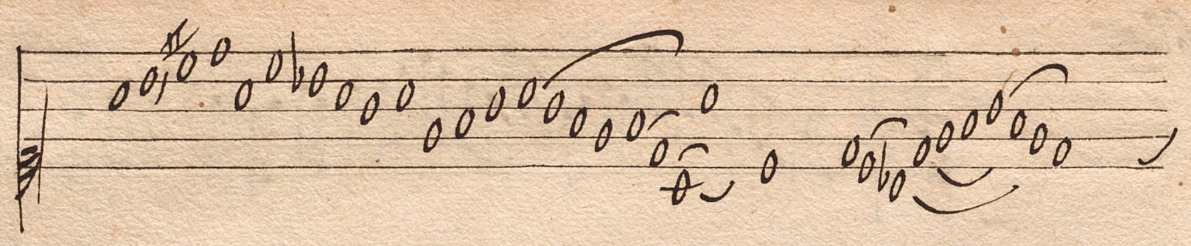
\includegraphics[width=.9\linewidth]{images/chapter1/delanglebert1.png}}
            \captionsetup{width=.5\linewidth}
            \caption[An excerpt from one of Jean Henry D'Anglebert's seventeenth-century unmeasured preludes using the ``whole note'' glyph to represent each pitch ametrically.]{An excerpt from one of Jean Henry D'Anglebert's seventeenth-century unmeasured preludes using the ``whole note'' glyph to represent each pitch ametrically.\footnotemark}
            \label{fig:nonmesure}
        \end{figure}
            \footnotetext{\fullcite{Chung_2019}}

    Thus, our second working definition:

        \begin{smallquote}
        An \textit{``open'' notation} is any notation which requires active creative (i.e. generative) participation on the part of an interpreter to faithfully render the musical product toward which it is oriented.
        \end{smallquote}

    %There is no clearly delineated fact-of-the-matter as to how the ``open'' parameters of the excerpt are to be played. 

    Note that this is \textit{not} to say that these open parameters were, in the seventeenth century, fully unbounded and that any interpretation would suffice, so long as it heeded the aforementioned fixed elements. Rather, ``openness'' in the most generic sense merely points to some degree of indefiniteness or ``incompleteness'' as regards what music, precisely, is represented on the page. Thus, crucially, under this view \textit{every} music notation designed for human interpretation is, in a non-trivial sense, open to some degree. Even the most seemingly stringent and exquisitely detailed forms of notation we find used by the likes of Brian Ferneyhough or Michael Finnissey necessarily leave key aspects of performance up to the taste and experience of the performer.
    
    Ian Pace, in his contribution to \textit{Unfolding Time} (2009), reinforces this notion via his ``negativistic'' account of music notation.   

        \begin{smallquote}
            [The historical construct of music notation \textit{in toto}] is, to my mind, founded upon an essentially \textit{positivistic} view of the role of notation. By this I mean the notion that the score tells the performer in essence \textit{what} to do, around which he can elaborate [...] depending on the degree of notational exactitude. The alternative model I wish to propose draws upon structuralist thinking about language; instead of seeing the score in a \textit{prescriptive sense} [...] I would suggest that instead it delineates the range of possible performance activities by telling the performer what \textit{not} to do. [...]

            \vspace{7pt}
            
            \noindent[I]f a performer thinks of notation in this way, the task becomes less one of playing something `right' as playing it `not wrong'.
        \end{smallquote}

    In short, the boundaries notation imposes on performance are in fact broad zones of exclusion. Per Pace's example, the triplets in Chopin's \textit{Impromptu in G$\flat$}, Op. 51 are fundamentally open in the sense that they permit any interpretation not excluded by their ``triplet-ness.'' Only if a performance departs so greatly from the printed page that the gesture is heard as an entirely different metric grouping does it qualify as unfaithful or ``incorrect''---thus, for Pace, a less detailed notation is a more open notation on account of forbidding fewer interpretations.\autocite[154--6]{Pace_2009} Crucially, though, there is no point of maximum fixity at which \textit{all interpretations but one} are forbidden; ergo, it is possible to meaningfully describe any notation as occupying some point along this axis.
    
    % Per Charles Seeger, the notation to which we are accustomed ``...does not tell us as much about how music sounds as how to make it sound. ... [N]o one can make it sound as the writer of the notation intended unless in addition to a knowledge of the tradition of writing he has also a knowledge of the oral (or, better, aural) tradition associated with it...''\autocite{Seeger_1958}

    For the purposes of this chapter, I'll dub the entire range from some purely theoretical fully-fixed, wholly representative notation to an equally hypothetical fully-open notation the ``fixity gradient.'' While each notation practice examined here will demonstrate fixity/openness in different ways and to different ends, this ``gradient'' might serve as a helpful (if reductive) analytic tool to facilitate greater insights into the way various notations mediate musical performance.

    \section{Notation as archive: Guido d'Arezzo's new fixity}

    We now largely conceive of liturgical notation in medieval Europe as gradually congealing into the four-line-staff form put forward by Guido d'Arezzo in the eleventh century, having originated in pitchless neumes which offered to the cantor only a general notion of melodic contour and syllabic stress.\autocite[16]{Taruskin_2009} While Guido was not the first to take a stab at more precisely encoding sacred melodies using ``heighted'' tones oriented around a central pitch (a practice which, in some form or another, dates at least as far back as Boethius and the ancient Greeks before him\autocite[17]{Taruskin_2009}), Guido's four-line staff facilitated melodic acquisition by allowing singers to more easily visualize the various intervals to be sung and to determine the chant's ``home'' hexachord.\autocite[53]{Reisenweaver_2012} Figure~\ref{fig:guidonew} shows one of a number of techniques Guido demonstrates in the \textit{Micrologus} which more precisely encode melodic contour. While often pitches would be appended to individual syllables, this rendering is looser still in that it gives the cantor no indication of syllabic break-points. The rhythmic indications shown in the inset mensural notation are an anachronistic appendage by a later publisher.

        \begin{figure}
            \centering
            \fbox{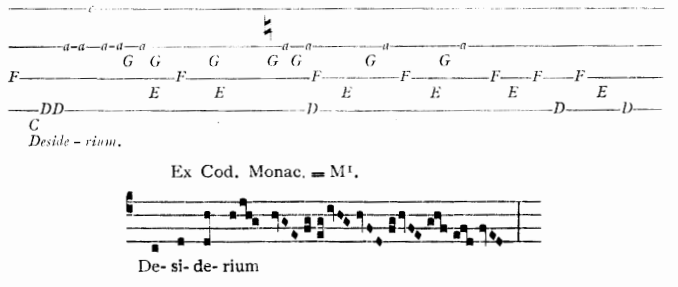
\includegraphics[width=.9\linewidth]{images/chapter1/guido4.PNG}}
            \captionsetup{width=.5\linewidth}
            \caption[A pedagogical excerpt from Guido's \textit{Micrologus} demonstrating the four-line staff with ``heighted'' neumes---shown here both in Guido's original letter notation (above) and in the later ``black note'' mensural notation (added in the 1904 Solesmes edition).]{A pedagogical excerpt from Guido's \textit{Micrologus} demonstrating the four-line staff with ``heighted'' neumes---shown here both in Guido's original letter notation (above) and in the later ``black note'' mensural notation (added in the 1904 Solesmes edition).\footnotemark}
            \label{fig:guidonew}
        \end{figure}
            \footnotetext{\fullcite[28]{Guido_1904}}

    Speaking generally, it was a centuries-long yearning for greater notational fixity---a more substantive relationship between sign-system and sound concept---that motivated this shift from pitchless to pitched neumes. Guido's stated goal, that ``anyone, with the use of the monochord and with careful instruction in the use of our notes, might, at the end of one month, be in a position to sing songs neither seen nor heard before, on the first glance''\autocite[16]{Arezzo_1943} arose explicitly in response to a perceived lack of accuracy in the recitation of traditional music, where previously even ``a hundred years [of] study of songs''\autocite[17]{Arezzo_1943} was insufficient to guarantee fidelity among learned singers.

    %[QUOTE ON NEED FOR NOTATION FROM TARUSKIN]
    %[PG 15 of original BPL194 manuscript: https://digmanclass.universiteitleiden.nl/manuscripts/bpl-194/] = guido2sancte

    In contrast to prevailing forms of concert music notation today, Guido's appears startlingly vague. His novel system (which would reach maturity in the form of the more complex ``black note'' mensural notation of the European Renaissance) demonstrates no rhythmic fixity whatsoever, owing, presumably, to the fact that these melodies were necessarily appended to sacred texts which carried with them their own prosodic rhythms. Similarly we find no specifics regarding pace, quality of voice, number of performers, ornamentation, etc. Referring to his treatise (but applying equally to his newly-developed system), he writes: ``That which in music is of little significance for the art of singing, or which would not be easily understood I have not held worthy of mention.''

    %[[CHANGE THIS SECTION --- FROM GUIDO OF AREZZO AND HIS INFLUENCE ON MUSIC LEARNING]]

    %Figures 2 and 3 below show one of a variety of techniques Guido demonstrates in the \textit{Micrologus} which precisely encode melodic contour\footnote{In this instance Guido is using this \textit{Sancte Iohannes} passage to illustrate one means of illuminating arbitrary liturgical texts using their vowel content}. The highlighted passage appends fixed pitches to each syllable of the text, which are then ``heighted'' to regular degrees above an initial pitch ``C.''

    The extent to which this system appears ``open'' by today's standards, though, should not be taken as an indication that its performers were granted a commensurate degree of creative latitude in its realization. Whereas deliberately open notations in the twenty-first century often serve as tacit invitations on behalf of a composer to bend the finished work to the performers will and experience, Guidonian notation was, from the outset intimately bound up with a robust o/aural tradition oriented toward regular, faithful reproduction of comparatively immutable sacred texts. So rigid and commonly-understood was this tradition, apparently, that Guido saw no need to render details of its execution in his notation, save for the melodies themselves which, on account of their prodigious quantity and the difficulty of their memorization, formed the main pedagogical stumbling-block of his project. 

    Perhaps owing to the notation's aforementioned lack of fixity, regional variation \textit{is} assumed to have cropped up as the new system moved geographically outward.\autocite[466]{Hucke_1980} Additionally, the question of varieties of rhythmic interpretation of plainchant melodies is far from settled. Attempts to uncover ``\textit{the} authentic rhythm of chant''\autocite[319]{Brunner_1982} have largely come up empty, inviting the notion that rhythmic variations between performances formed much of the regional flavor of church music practice. However, this variation clearly arose by virtue of the notation's ``technological'' limitations and the realities of pre-Enlightenment communication rather than from some desire on the part of the notation's architect(s) to draw out these distinctions. Arguably, the miracle of Guidonian notation and its successors lies in the fact that despite such sparse notation, the genre underwent precious little change (melodically, at least) over centuries of practice---perhaps, as Helmet Hucke argues, because chant manuscripts quickly became more of a ``control against deviation from the true and venerable tradition'' than specifically performance or pedagogical aids.\autocite[448]{Hucke_1980}

    To be clear, neither the fixity of a system of notation nor the historical steadfastness of its resulting melodies preclude creative musicianship via forms of improvisation. \textit{Micrologus}' controversial Chapter XVII takes pains to describe a method by which a student might improvise a new chant on a given text using the structure of its vowel content, gradually presenting the student with more and more melodic liberties as the lesson unfolds. Singers attempting this process are encouraged to ``[take] the preferred from the many attempts, [choose] the most pleasing way, [fill] up the cracks, [enlarge] the group, [have] them all moving together [...] so that one gets the most highly unified work possible.''\autocite[70]{Arezzo_1943} Improvisation, for Guido, is not valued for its ability to create \textit{many} valid instances of a work from \textit{one} central score-artifact, but rather its ability to achieve the most euphonous single work via a process of repetition; of trial and error. In a way, this procedure complicates the distinction between ``text'' and ``score'' insofar as he  purports to be able to unlock melodies already present within the text's syllabic content---thereby rendering each text-sans-melody ``always already'' a symbolic system pointing toward a fixed sound world. The only distinction between this text-score and notation as traditionally understood is the process by which the sound-world is unlocked: in this case, through the process of improvisation itself.

    In sum, Guido's efforts to bring greater fixity to the practice of notating existing liturgical works succeeded beyond what he could have possibly imagined in two ways: first, in that they persist (albeit in a modified form) to this day in the canonical collection of Roman Catholic chants, the \textit{Liber Usualis}, and second, in that they provided the basis for the succeeding thousand years of concert music notation and all variants thereof. Further, despite the appearance (through modern eyes, at least) of a great degree of openness in the earliest ancestors of western notation, the symbols' tethers to a particular sound-concept were really rather fixed insofar as they were tightly regulated by a tradition of liturgical practice. As we shall discuss soon, only when musicians begin to make the critical shift from using scores as mnemonic aids and regulatory standards to actual \textit{performance} tools do we begin to see notation's openness mediate musicianship in ways more familiar to the twenty-first-century musician.

    % \begin{notestuff}
    %     I may end up grouping together my own broader commentary in a separate section following summary, so this may be moved later.
    % \end{notestuff}

    %[QUOTE ON FIXITY OF LITURGICAL CHANT -- despite open notation...]

    %[the question of rhythm in old chant notation is not a settled one!! it's a thorny problem -- see "The Performance of Plainchant: Some Preliminary Observations of the New Era'']
        
        
\section{Score-mediation in \textit{cantare super librum}}

   % \begin{notestuff}
   %     Just rephrase this first couple of sentences---it's my idea, so make that crystal clear (and maybe convince the reader it's a sound idea).
   % \end{notestuff}

    Insofar as its relationship to notation is concerned, the first major sea-change in Western music arrives only when printed musical materials begin to function not only as archival or pedagogical artifacts but as tools which facilitate performance itself. By the fifteenth century, inscribed musical works now have the ability not only to cement the products of an oral tradition for pedagogy and posterity, but also, increasingly to \textit{liberate} musicians from the onus of memorization; instead directly affording them musical techniques to employ in performance Openness here is still strictly mediated by the vagaries of good taste, tradition, etc., though now there is a new expectation of literacy: namely, that a performer should be able to, in real time, transform some ``unfinished'' skeletal framework (read: a bare melody of some kind) into a florid ``finished'' work.

    This change---really a very gradual series of non-localized changes---coincides with the growing sense of the independent existence of the musical artwork unto itself: the development of the work-concept. More sophisticated notation, claims Laurenz Lütteken, imparts new stability to canons of musical work, allowing musical practices to develop associated bodies of literature. This consequently permits the rise of the inexorably linked twin practices of music theory and literate composition.\autocite[57]{Lutteken_2020} Richard Taruskin, too, notes the historical import of new literate musical practices in the fifteenth century, arguing that ``the earliest manifestation of the condition of `absolute' art or art-for-art's-sake'' coincides with the rise of more sophisticated polyphonic practices and the more widespread distribution of the same---developments which would hardly have been possible without the technological refinements of new notation: a robust means of inscribing music's rhythm/meter; collections of non-texted songs, applicable to both vocal and instrumental performance; etc.\autocite[541]{Taruskin_2009}

    Of these new literate musics which emerge during the Renaissance, the (still predominantly liturgical) practice of \textit{cantare super librum} serves as the most poignant example of a notation-mediated open music. Specifically, it requires both a familiarity with the symbols used to encode the melodic framework of a piece of music as well as the creative strategy by which a player might ``see through'' the notation to the field of improvisatory potential implicitly permitted by the symbolic system. To wit, \textit{cantare super librum}\footnote{Translated ``singing over the book''---i.e. \textit{contrapunto concertado}, \textit{contrapunto alla mente}, \textit{chant sur le livre} depending on country of origin.}---a technique first described by Tinctoris in his 1477 treatise \textit{Liber de arte contrapuncti}---describes a process by which a group of singers, song-books in hand, spontaneously generate a polyphonic composition in two, three, or more parts using a melodically/rhythmically fixed cantus firmus as a ground which persists across performances. This practice serves as the \textit{ne plus ultra} literate collective-improvisatory music of the fifteenth century. 

    % \begin{notestuff}
    %     I can probably relegate this fauxbourdon stuff to a footnote and omit the figure if I want to. It's not really doing any good here.
    % \end{notestuff}

    % To anticipate a potential objection: The practice of \textit{fauxbourdon} whereby, broadly, singers added parallel consonances in rhythmic isochrony to a cantus firmus, similarly required both musical literacy and some degree of extemporization.
    %     \footnote{
    %         Here, for the purposes of space I'm using the term \textit{fauxbourdon} as shorthand for what is actually a wide variety of techniques (see also: faburden, \textit{falso bordone}) which are all distinct but which share important familial similarities.
    %     }
    % (Figure~\ref{fig:fauxbourdon} provides a paradigmatic example.) These techniques were practiced concurrently with \textit{cantare super librum}, but also preceded its use in the church by many, many years and thus might also be considered a hinge-point in our collective relationship to open notations. However, while the precise intervallic relationship between the cantus, tenor, and other voices differed geographically and by era, within a given \textit{fauxbourdon} tradition, these relationships were more or less static, and only rarely departed from their stolid, homophonic note-against-note texture.\autocite[434-7]{Taruskin_2009}

    % \begin{figure}
    %     \centering
    %     \fbox{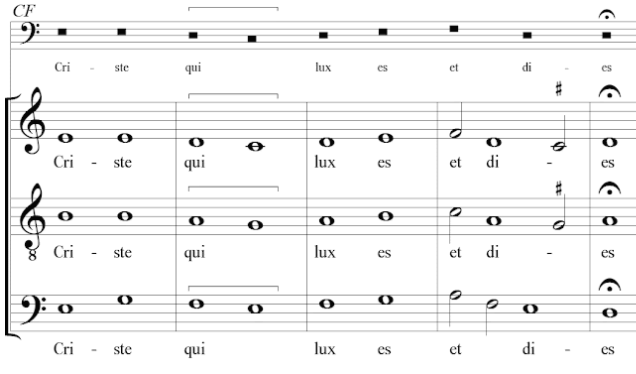
\includegraphics[width=.8\textwidth]{images/chapter1/fauxbourdon1.PNG}}
    %     \captionsetup{width=.5\textwidth}
    %     \caption[An excerpt demonstrating one \textit{fauxbourdon} harmonization variant over a fixed cantus firmus. Note rhythmic isochrony and predominantly fixed intervallic relationships between voices.]{An excerpt demonstrating one \textit{fauxbourdon} harmonization variant over a fixed cantus firmus. Note rhythmic isochrony and predominantly fixed intervallic relationships between voices.\footnotemark}
    %     \label{fig:fauxbourdon}
    % \end{figure}
    %     \footnotetext{\autocite[]{Rotem_2022}}

    % These universally stringent rhythmic and melodic ties to the cantus firmus rather strictly delimited the creative latitude afforded to any one practitioner. ``Improvisation'' such as it is in this context is token at best when compared with later, more sophisticated forms of truly polyphonic performance. As such, I consider \textit{fauxbourdon} less a fully-fledged open form and more a stylistic stepping-stone toward the sorts of open music practices which concern this research.

    In contrast with other (earlier and contemporary) literate musics, \textit{Cantare super librum} clearly required a more robust sense of a desired aesthetic for the final work insofar as each participant was required to heed principles of good taste in their use of rhythmic motifs, melodic structure, cadences, etc., in effect each creating an independent contrapuntal voice in real time.\footnote{
        To anticipate a potential objection: The practice of \textit{fauxbourdon} whereby, broadly, singers added parallel consonances in rhythmic isochrony to a cantus firmus similarly required both musical literacy and some degree of extemporization. These techniques were practiced concurrently with \textit{cantare super librum}, but also preceded its use in the church by centuries. As such, \textit{fauxbourdon} might fairly be considered a hinge-point in Western notation worthy of inclusion in this survey. However, while the precise intervallic relationship between cantus, tenor, and other voices differed geographically and by era, within a given \textit{fauxbourdon} tradition, these relationships were more or less static, only rarely departing from their stolid, homophonic note-against-note texture. (\autocite[434--7]{Taruskin_2009}) Thus, while there was no doubt some degree of extemporization (embellishments, cadences, etc.), \textit{fauxbourdon} rather strictly delimited the creative latitude afforded to any one practitioner. ``Improvisation'' such as it is in this context is token at best in contrast with later, more sophisticated forms of authentically polyphonic performance. As such, I consider \textit{fauxbourdon} less a fully-fledged open form and more a stylistic steppingstone toward the sorts of open music practices which concern this research.
    }
    As such, the practice also necessitated a greater ability to ``see through'' the open skeletal framework provided by notation into (what we'll dub) the ``field of musical potential'' --- i.e. the network of musical moves available to a performer which fulfill the demands of the work-concept as it is understood.

        \begin{figure}
            \centering
            \fbox{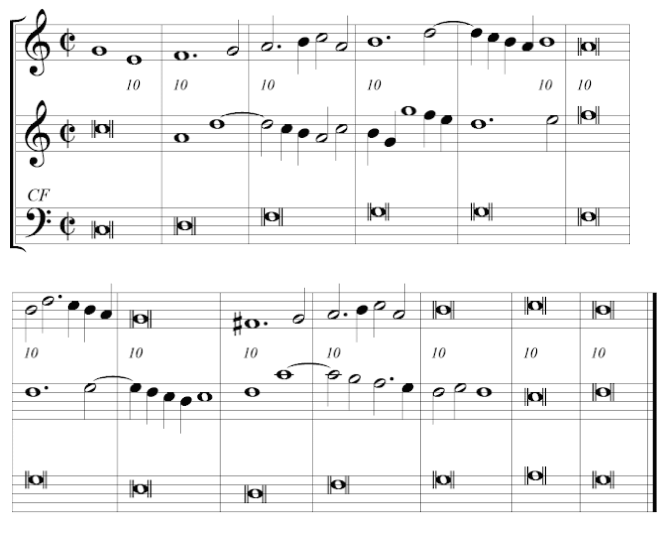
\includegraphics[width=.8\textwidth]{images/chapter1/cantaresuperlibrum1.png}}
            \captionsetup{width=.5\textwidth}
            \caption[A hypothetical contrapuntal ``illumination'' of a cantus firmus realized in a \textit{cantare super librum} style, per later sixteenth-century Italian pedagogical manuscripts.]{A hypothetical contrapuntal ``illumination'' of a cantus firmus realized in a \textit{cantare super librum} style, per instructions elucidated in later sixteenth-century Italian pedagogical manuscripts.\footnotemark}
            \label{fig:cantare}
        \end{figure}
            \footnotetext{\autocite[]{Rotem_2022}}

    Figure~\ref{fig:cantare} above is, of course, only a hypothetical example, helpfully constructed using contemporary sources by early music scholar Elam Rotem. Though presumably the occasional masterpiece extemporization was transcribed for posterity, as with all improvisatory practices the vast, vast majority of \textit{cantare} realizations have been lost to time. While methods varied greatly across Europe during the fifteenth century, certain techniques like the embellished ``parallel tenths'' model shown in the figure turn up frequently enough to be identified as a core improvisational strategy.\autocite{Rotem_2022} Pedagogical treatises, like those of Johannes Tinctoris and his descendants, can give the modern reader a sense of what it must have been like to engage with a cantus firmus \textit{qua} open notation. Universally, these manuals present the reader with potential contrapuntal embellishments---solutions to various intervallic scenarios which over time become familiar enough to the student that recognized patterns in liturgical melodies begin to afford these embellishments directly in performance. Figure~\ref{fig:lusitano} illustrates three such bite-sized affordances. In the first of these, a stepwise descent in the bass from D to C presents the possibility of a symmetrical stepwise ascent of a 7th in a particular rhythmic pattern. The second shows the inversion of the first, and the third demonstrates a more complex solution over a longer cantus segment. To the fifteenth-century improvising cantor, the aforementioned ``field of musical potential'' which avails itself \textit{via} the unadorned cantus firmus comprises a sort of networked map, itself comprising countless such embellishments, harmonizations or diminutions---first learned by rote then ``forgotten.''\footnote{(to borrow a turn of phrase perhaps apocryphally ascribed to Charlie Parker)}

        \begin{figure}
            \centering
            \fbox{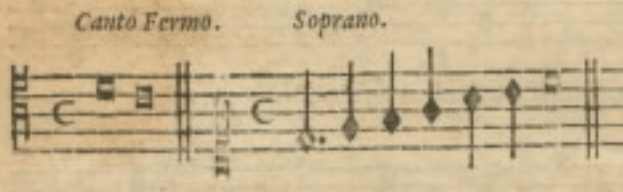
\includegraphics[width=.5\textwidth]
            {images/chapter1/lusitano1.png}}
            \fbox{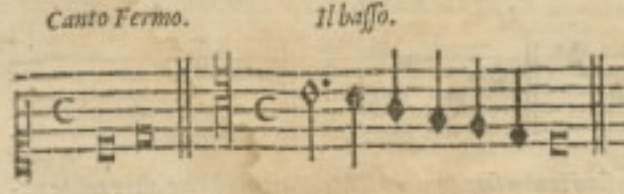
\includegraphics[width=.5\textwidth]{images/chapter1/lusitano2.png}}
            \fbox{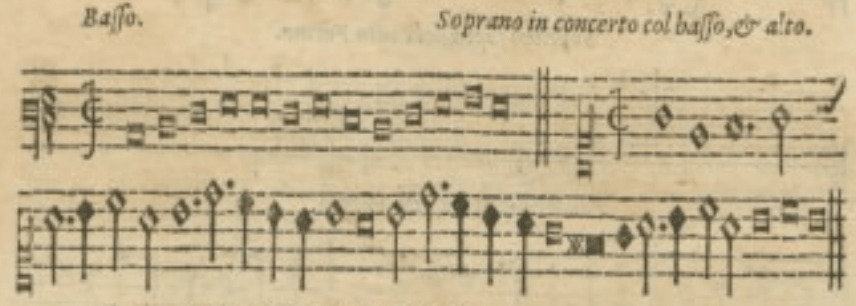
\includegraphics[width=.7\textwidth]{images/chapter1/lusitano4.png}}
            \captionsetup{width=.5\textwidth}
            \caption[Pedagogical ``sample'' realizations of short cantus firmi, from Vicente Lusitano's 1553 treatise \textit{Introduttione facilissima}.]{Pedagogical ``sample'' realizations of short cantus firmi, from Vicente Lusitano's 1553 treatise \textit{Introduttione facilissima}.\footnotemark}
            \label{fig:lusitano}
        \end{figure}
            \footnotetext{\autocite[15]{Lusitano_1561}.}

    It is my contention that the fundamental (``phenomenological,'' if you like) experience of the \textit{cantare super librum} improviser is, despite the vast historical gulf separating them, predominantly similar to the experience of later notation-mediated improvising musicians, be they continuo harpsichordists or bebop trumpet-players. In each case, a musician has the ability to ``acquire'' a skeletal compositional form via notation (one which, if rendered ``directly''---i.e. played note-for-note---would represent a hopelessly impoverished example of the work itself) which they are then expected to illuminate via a series of embellishments or wholesale inventions mediated by strictures communicated by the form itself. These written forms, of course, vary in the degree of detail they express; that is, in the closeness with which their symbolic systems correspond to the finished product (their \textit{fixity}). The performer here constantly negotiates between the printed material, their personal ``field of musical potential'' acquired via training and experience, their commitments to the performance scenario (e.g. ``Is this realization appropriate to this time/place/work?''), and, arguably, their sense of artistic identity (e.g. ``Does this realization adequately represent \textit{me} as an artist?'').

    Of course, each musician operating in these disparate genres bears a different, personal relationship to notation itself---indeed, there have been exemplary figures in every era who reach astounding levels of improvisational sensitivity despite being musically ``illiterate.'' Musician-to-musician and teacher-to-student o/aural transmission have, in all cases, formed a crucial component in the building of these ``fields'' of potential musical moves. To again cite Laurenz L\"utteken, ``[m]usic does not need to be fixed or transmitted in written form to constitute a work'' and neither must musicians necessarily engage with score-artifacts in order to take part in their associated literate traditions.\autocite{Lutteken_2020} However, contrary to all-too-prevalent attitudes that notation somehow ontologically lags behind music making proper, parasitically dependent on o/aurality for its very existence, I share Floris Schuiling's view that notations themselves ``serve to construct forms of musical interaction [...] offer[ing] different ways of imagining sound as music, make different demands on musical knowledge, and condition musicians' creative agency.''\autocite[431]{Schuiling_2019} As such, the notion that (western) music notation is inevitably downstream from somehow ``purer'' acts of music making is, in my view, untenable. When a notational practice (predominantly open or otherwise) is so inextricably integrated with the learning, dissemination, and reification of musical works, there is a very real sense in which even the musically ``illiterate'' still engage, by proxy, with structures of notation. 

    Even insofar as a musician might ``graduate'' from the printed page--- becoming so familiar with an oft-repeated work that s/he no longer needs to physically peer at its skeletal frame---s/he still renders the work in real time using sound-concepts that are best and most often expressed in the system of notation surrounding the work's associated corpus. To reiterate: I take it that this relationship between musician and notation (i.e. between artist/artisan and material) constitutes a style of notational mediation which permanently refigured the nature of (western art) music-making and which, in essence, still constitutes a large part of the experience of modern musicians today. 
    
    % \begin{notestuff}
    %     Per a comment from Amy, I think I'll reorganize this section a bit, adding in one or two contemporary sources (one or two figured bass manuals advocating for particular sorts of improvisatory performance) and relocate my commentary to a later section.
    % \end{notestuff} 

    In sum, the fifteenth century represents a crucial locus for the development of modern notational practices. First, it sees the rise of a mature mensural notation; one which records both absolute pitch and proportional durational values using a far more robust encoding scheme than in previous generations. Second, the way notation is used in the fifteenth century begins to resemble contemporary usage to a much greater extent in that it gains performative rather than strictly archival/pedagogical utility. The preponderance of theoretical treatises written during this period as well as the new flourishing of complex (written) works which approach composition from a ``notation-first'' perspective demonstrate that key aspects of the notion of literacy so central to Western art music today were in full swing over half a millennium ago.\footnote{See, for instance, Ockeghem's experimental \textit{Missa Prolationum} which arguably centers the \textit{manipulation of a symbolic system} as its main compositional process over and above merely crafting a beautiful, genre-appropriate sound-world.} 

    There is a very real sense in which fifteenth-century Western notation (particularly notation employed in expressly improvisatory genres like \textit{cantare super librum}) utterly relies on its openness. The notion that a piece of music could somehow be ``fully represented'' by its score or parts is fundamentally incompatible with the way written music was performed during this era---whether primarily improvised or merely ornamented. Much like the more recent examples of open/literate music-making to be described in later sections, the fifteenth-century musical work-concept only forms at the nexus of composer, performer, and score-artifact---a relationship mediated in no small part by the nature of the symbols themselves.
    
   % \begin{uselater}
   %     ...what remains is for composers to begin deploying purpose-built tools to wield + change the performer's improvisatory capabilities.
   % \end{uselater}

\section{Post-fifteenth-century reforms in open notation}
   
     %\paragraph{\textit{Basso continuo} and figured-bass}
     Above, I argued that the experiential kernel at the heart of open/literate music performance began, in essence, with improvisatory fifteenth-century polyphony. Of course, this is not to say that the intervening centuries between the fifteenth- and twenty-first did not see their share of important development in the art of open notation. Making its first documented appearance in the literature via a Roman manuscript in 1600, the practice of figured \textit{basso continuo}---likely far more familiar to modern readers than \textit{cantare super librum}---would become arguably the most prevalent and durable open notation in Western art music, representing one of the richest examples of a highly o/aural yet strongly notation-mediated performance practice in the literature.\autocite[811]{Taruskin_2009} Though, to be clear, this chapter lacks the space for any truly detailed treatment of the topic, it should suffice for future comparisons to briefly gloss its novel open notation scheme.

    In essence, \textit{basso continuo} refers to both (a) an inscribed bass line and concomitant harmonic structure which, together, undergird a (typically Baroque) performance and (b) the performance practice itself. While frequently used to notate accompanimental sub-ensembles, it crops up often in pieces for unaccompanied homophonic instruments (organ, lute, harpsichord, etc.). Given that \textit{basso continuo} flourished for over 150 years, the technique appeared with many variations according to local convention, though all share a composer-provided bassline (meant to be performed as-written with little variation) and some means of encoding operant harmonies over which the performer improvises according to certain constraints. Though in modern parlance the term is frequently interchanged with ``figured-bass,'' instrumental improvisation over basslines of the \textit{continuo} form long preceded the development of the accompanying numeric figurations. To be precise, Marla Hammel locates the origin of un-figured \textit{continuo} \textit{avant la lettre} in the aforementioned early polyphonic music of the Catholic church. Figured-bass proper, on the other hand, began in Rome and quickly spread outward owing to its many advantages over the more opaque un-figured variety.\autocite[28--9]{Hammel_1977}

    Jeffery Kite-Powell elaborates in his \textit{Performer's Guide to Seventeenth-Century Music}: 

        \begin{smallquote}
            The idea of adding a chordal accompaniment to vocal or instrumental pieces had been practiced in one way or another for over a century, either by improvisation or by reading ``short score'' [...] but the practice grew with special intensity in the declining years of the sixteenth century as musicians began writing---and publishing---such music in the convenient method of figured (and unfigured) basses. As the practice spread, it was applied to older-style polyphonic textures, as well as to the newer ones of solo melody.\autocite[317]{Kite-Powell_2012}
        \end{smallquote}

    This ``shorthand'' most often takes the form of numeric figuration beneath the given bassline (of the form $^{5}_{3}$, $^{4}_{2}$, $^{\sharp6}$, etc.) which, at a minimum, indicates to a performer which intervals are to be sounded above the bassline---usually without reference to a particular octave. More than mere stand-ins for un-notated tones, though, these numeric glyphs imply particular harmonic fields which in turn form the basis of the performer's improvisatory embellishments on the fundamental line. Figure~\ref{fig:figuredbass} gives a paradigmatic example of figured bass notation as used in Georg Philipp Telemann's violin sonata, TWV 41:F3 (1734) illustrating the soloist's melody with figured bass beneath.
    
      \begin{figure}
            \centering
            \fbox{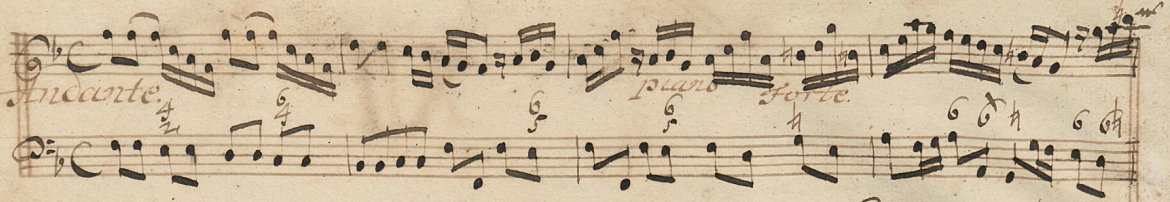
\includegraphics[width=.9\textwidth]{images/chapter1/telemann1.png}}
            \captionsetup{width=.5\textwidth}
            \caption[A paradigmatic sample of figured bass notation from Telemann's violin sonata TWV 41:F3. Drawn from a contemporary manuscript.]{A paradigmatic sample of figured bass notation from Telemann's violin sonata TWV 41:F3. Drawn from a contemporary manuscript.\footnotemark}
            \label{fig:figuredbass}
        \end{figure}
            \footnotetext{\fullcite[]{Telemann_1734}}

    To appropriately realize a figured-bass passage is to delicately balance \textit{recitation}, i.e., recreating the specified bassline and intervals above, and \textit{creation}, i.e., ``seeing through'' the simple figures to the implied harmonic function and reinforcing it through improvisation. Of course, this raises new questions: If earlier, un-figured lines were sufficient to improvise ``over the book'' or to provide accompaniment to a soloist, then why was it necessary to conceive and deploy an entirely new set of glyphs---i.e. yet another system to teach and to memorize? And what significance do these new symbols have to the relationship between performer and score if performers were getting on well enough without them? 
    
    In essence, figured \textit{continuo} was a labor-saving device; a novel musico-graphic technology. The skills required to quickly examine a number of vocal or instrumental parts (or even a lone bassline) and extract enough salient harmonic information to cogently improvise behind an ensemble required extensive training: time and money. These figurations allowed a composer to much more efficiently and precisely communicate a piece's harmonic structure to a would-be improviser while also allowing less-musically-literate performers the opportunity to meaningfully participate in otherwise inaccessible music. Though the degree of figuration provided would differ according to time, place, composer, and publisher, to the extent that they were present these figures lent performers more clarity and composers greater control of the otherwise thorny, opaque process of improvisational accompaniment.\autocite[321]{Kite-Powell_2012}

    Ultimately, I contend that \textit{basso continuo} still fundamentally upholds the \textit{cantare} model of composition/improvisation insofar as it is still ultimately left up to the performers' training and good taste to determine the authentic/appropriate bounds for their contributions. However, the introduction of a new, bespoke system for encoding harmonic information does represent an important turning point in Western notation. Specifically, it marks an early concerted effort to sculpt and/or facilitate the communication of the boundaries of improvisatory musicmaking. Musical glyphs had, since the fifteenth century at latest, been forced to pull double-duty in somehow representing not only the fixed parameters of performance but the open ones as well. Though figurations would never fully obviate performer expertise in sussing out these open parameters, they provided a simple graphic synopsis through which to conceptualize a work's changing harmonic field (and indeed even even harmony generally).
    
    %        \begin{uselater}
    %            Two more paragraphs here explaining how figured bass is the result of economic/sociological pressures---how they are coded communication from the composer to the performer that they're expected to improvise under constraints---that they represent a new VERTICAL conception of harmony---how I'll touch later on 20th-century chord symbols (and that they're basically the same thing) and that they're really interesting but I don't have the space. I should probably cite a pedagogical treatise which mentions the sorts of creative liberties afforded to the performer! Then do my little finishing paragraph at the end of the section. 
    %            
    %            In short, it grants composers more precision in sculpting their performers' improvisatory efforts; it facilitates pedagogy rather than hindering it; it allows the dissemination of musical materials to newly-literate groups of musicians. 
    %        
    %            Why is this relevant to narrative? Well, it's a concrete piece of notational technology invented to facilitate communication of the boundaries of improvisation.
    %        \end{uselater}
        
    
    %    A more detailed treatment of this topic would, no doubt, delve further into the increasing sophistication with which composers (for a variety of reasons) begin to incorporate open materials into their works in the ensuing centuries. First ``officially'' entering the literature via a Roman manuscript in 1600, the practice of \textit{basso continuo}---arguably the arch-open-notation in terms of its relative prevalence and durability---represents one of the richest examples of a strongly o/aural yet equally notation-mediated performance practice in the literature.\autocite[811]{Taruskin_2009} Further, its use of both a skeletal melody \textit{and} an associated ``vertical'' conception of harmony (new for the seventeeth century!) cements it as the tradition which bears the strongest resemblance to today's lead-sheet-mediated jazz performance, perhaps our most universally familiar literate open music practice. Figure~\ref{fig:figuredbass} gives a paradigmatic example of figured bass notation belonging to Telemann's TWV 41:F3. 

    As any student of music history is aware, though, this long, rich period of well-integrated literate/improvisatory practice was not to last forever. Certainly, the bulk of Western art music practiced today demonstrates a far scantier degree of interpretive latitude when it comes to score-reading. Robin Moore, in an essay titled ``The Decline of Improvisation in Western Art Music,'' sums up: Today, he claims, ``[t]he mandates of compositionally specified interpretation now supersede those of the instrumentalist. To many, improvisatory expression seems threatening, unfamiliar, or undeserving of interest.''\autocite[63]{Moore_1992} 
    
    Of course, despite the fact that the musical period marked by widespread \textit{continuo} practice is commonly thought of as the local apex of ``classical'' improvisation, this is not to suggest that improvisation in Western art music surreptitiously vanished at the end of the Baroque period. Eighteenth-century giants W. A. Mozart and Ludwig Beethoven are generally noted to have been skilled improvisers whose extemporizations often made their way into their finished works. Indeed, as Moore continues,

        \begin{smallquote}
            Even well into the 19th century it is clear that improvisation remained an indispensable ability for most professional musicians. We know that Brahms, Paganini, Chopin, Clara and Robert Schumann, Mendelssohn, Hummel, Cramer, Ries, Spohr, Joachim, and Schubert, to cite a few familiar names, were all accomplished improvisers in addition to composers and/or performers of precomposed music.
        \end{smallquote}
    
    \noindent Further, systematized improvisatory styles waxed and waned in intervening centuries. French liturgical organ music, for instance, saw increasingly codified improvisation throughout the eighteenth and nineteenth centuries, expounded upon by contemporary scholar-pedagogues like Alexandre-Étienne Choron\footnote{\textit{Sommaire de l'Histoire de la Musique} (1810)}, François-Joseph Fétis\footnote{\textit{Méthode élémentaire de plain-chant à l'usage des séminaires, des chantres et organistes} (1843)}, and their heirs Louis Niedermeyer and Joseph d'Ortigue\footnote{\textit{Gregorian Accompaniment: A Theoretical and Practical Treatise Upon the Accompaniment of Plainsong} (1856--7) (helpfully available in English, translated by Wallace Goodrich)}, François-Auguste Gevaert\footnote{\textit{Méthode pour l'Enseignement du Plain-chant et la Manière de l'Accompagner, Suivie de Nombreux Exemples} (1856)}, and Jacques-Nicolas Lemmens.\footnote{\textit{Du Chant Gregorien, sa Melodie, son Rythme, son Harmonisation} (1886 posth.)}

    These improvisatory practices, however, differ from those of the Baroque and Renaissance in one critical sense. Rather than make use of yet more sophisticated notations-for-improvisers, they instead (in a sense) retrogress. As the eighteenth century wears on, music begins to become more and more fixed-in-place on the score: where improvisation occurs, it occurs \textit{contra} the score rather than through it. The next section of this chapter will briefly attempt to account for this historical waning of open-notation-centric performance models and the turn toward yet greater degrees of notational fixity in the late-eighteenth and nineteenth centuries.

        %\begin{uselater}
        %    Argue that FB was basically the apex of open/literate music but concede that it wasn't totally static. Maybe this couple of paragraphs could just be merged into the next section.
        %\end{uselater}
        %
        %    \begin{notestuff}
        %        I should rephrase the following paragraph. Concede that things did change but that for the purposes of our larger-scale ``ebb-and-flow'' narrative, the most significant changes in Western music notation came with the concretization of the work-concept during the galant. It's what I'm going into in the next section, so I just need to signpost that discussion.
        %    
        %        Something like:
        %    
        %        While further discussion of these smaller-scale developments in Western notation-mediation is long overdue, the space allotted here is unfortunately insufficient to do any serious work here. On the larger scale...
        %    \end{notestuff}
   
    %    \paragraph{Other open/literate musics} Especially in France, various styles of improvisation at the organ, too, developed in intervening centuries. These are expounded upon in treatises by eighteenth- and nineteenth-century writers such as Alexandre-Étienne Choron\footnote{\textit{Sommaire de l'Histoire de la Musique} (1810)}, François-Joseph Fétis\footnote{\textit{Méthode élémentaire de plain-chant à l'usage des séminaires, des chantres et organistes} (1843)}, and their heirs Louis Niedermeyer and Joseph d'Ortigue\footnote{\textit{Gregorian Accompaniment: A Theoretical and Practical Treatise Upon the Accompaniment of Plainsong} (1856--7) (helpfully available in English, translated by Wallace Goodrich)}, François-Auguste Gevaert\footnote{\textit{Méthode pour l'Enseignement du Plain-chant et la Manière de l'Accompagner, Suivie de Nombreux Exemples} (1856)}, and Jacques-Nicolas Lemmens.\footnote{\textit{Du Chant Gregorien, sa Melodie, son Rythme, son Harmonisation} (1886 posth.)} These methods of plainchant accompaniment, though distinct, likewise involve a similar ``deep'' literacy as regards the illumination of sparse, open printed materials---which may take simpler forms (adding isochronous, vertical harmonizations below a chant, for example) or more complex ones (full, multi-voice counterpoint which sequesters the original chant somewhere in an inner voice).

    %Bracketing further discussion of these and other fascinating examples of the flourishing of open notation, it must suffice for now to stake out the claim that (insofar as said notation is concerned), players' overarching musical roles underwent no massive paradigm shift between the mid-fifteenth century and, say, the galant period ending in the late eighteenth century. It is clear, though, that \textit{unlike} practices of literate improvisation or other creative musical interpretation during this long historical era, Western art music as practiced today (barring post-1970 changes which we'll discuss presently) features a far scantier degree of interpretive latitude when it comes to reading music. Per Robin Moore, ``The mandates of compositionally specified interpretation now supersede those of the instrumentalist. To many, improvisatory expression seems threatening, unfamiliar, or undeserving of interest.''\autocite[63]{Moore_1992} The next section of this chapter will briefly attempt to account for this historical waning of open-score-centric performance models and the turn toward yet greater degrees of notational fixity in the late-eighteenth and nineteenth centuries.
        
        %%%%%%%%%%%%%%%%%%%%%%%%%%%%%%%%%%%
        %%% LITTLE ORPHANED TOPICS %%%%%%%%
        %%%%%%%%%%%%%%%%%%%%%%%%%%%%%%%%%%%
        
        %It is clear, though, that \textit{unlike} the dominant art music paradigm with which we entered the twentieth century, that of the fifteenth century also demanded a different sort of literacy: namely, a well-developed relationship to open scores and familiarity with the processes by which they were to be brought to completion in performance. BIG CHANGES IN WHAT CONSTITUTES LITERACY
        
        %However, he is quick to point out that as of the fifteenth century, ``[n]otated compositions were treated as `works' in that they record[ed] how the music existed in performance, not insofar as they serve[d] as a prescriptive prompt for future presentation: the `work quality' inhered in the performance itself, not the written memento.''
        
        %\textcolor{red}{[of course, making positive claims about how music's openness was perceived/utilized at the time of its creation is nigh impossible -- but turning to contemporary performance guides can give us insight into the sorts of affordances notation carried with it. What sort of fields of sonic/action potential ]}
        
        %\textcolor{red}{
        %[The development of the work-concept in the fifteenth C.]
        %[Cantare Super Librum -- taruskin p.436-438]
        %[Prelude to figured bass -- structured improvisation based on a single melodic line]
        %[Diminutions as score-oriented improvisatory practice]
        %[First printed continuo -- taruskin p.811]
        %}
        
        %    \section{Openess in the common-practice period}
        %\textcolor{red}{
        %    [MAYBE CUT THIS SECTION ENTIRELY --  I THINK OPEN NOTATION EXPERIENCES ARE SIMILAR ENOUGH BETWEEN END OF RENAISSANCE AND COMMON-PRACTICE THAT WE COULD GO RIGHT TO ROMANTIC CONCRETIZATION]
        %    [Maturation of continuo practice -- resembling lead-sheets... but also the beginning of the end?] 
        %    }

    \section{Concretizing the sound-concept}
        
        % \begin{notestuff}
        % \begin{itemize}
        %     %\item \textcolor{red}{[Goal here is 99\% well-cited historical account and 1\% commentary.]}
            
        %      % \item Throughout this paper I have perhaps somewhat carelessly conflated ``improvisation'' (a term both extremely vague and hopelessly loaded) with the realization of notation of \textit{any} degree of openness. This is on purpose. I see no difference-in-kind between a long extemporization on a D-dorian chord/scale in the context of a jazz tune and the trivial decision to interpret a melodic fragment \textit{molto secco} rather than \textit{espressivo}... This might need some explanation though?? --- The rise of notational fixity == the closing off of the ``field of musical potential'' == more semantic content packed into each unit of notation
        
        %     %\item \textcolor{red}{Hammel cites ``the demise of partimento in Italy'' as a transition away from improvisation practices}
        
        %     %\item \textcolor{red}{There should be some attempt to track actual changes in the glyphs. Additions of more and more detailed dynamic markings, hairpins, etc., as well as articulations and expressive texts and specific tempo markings. --- Not to mention the decline of abbreviated embellishments (turn, mordant, etc)}
        
        %     %\item Beethoven's early works serve as another important hinge-point in their omission of the embellishments that characterized the prior 200 years or so...
        
        %     %\item Beethoven, of course, adds turns and trills into his music but these now serve more as a composer's shorthand---a notational device used to save ink rather than to inject a measure of improvisational spontaneity and freshness into an otherwise unchanging score.
        
        %     % \item ``...unwritten ornaments were still routinely employed and expected in Italian recitative as late as the 1850s, whereas many performers beginning in the 1880s took to `weeding them out' even in Mozart, reflecting a new literalism that affected the way in which notation was interpreted as soon as unwritten (`oral') traditions lost their sway in pedagogy. What was mistakenly viewed as the removal of inauthentic accretions was in fact a modernization.\autocite[591]{Taruskin_2009a}''\
        
        %     %\item ``In 1852, Johann Georg Meister made the sober assessment that `[h]armony and thoroughbass are therefore fairly equivalent in their meaning.\footcite[6]{Diergarten_2011}'
        
        %     %\item Certainly seems like some combination of more musicians = less time per musician to teach delicate improvisatory arts (teaching to read is far easier) + the adoption of German theoretical models in pedagogy over literate-improvisatory Italian partimento tradition...
        
        %     %\item (It's not only that notation simply took on a \textit{greater} role in music pedagogy/transmission, it's that notation was necessarily reduced to its simplest form---as representations of fixed aspects of a sound world.)
        % \end{itemize}
        % \end{notestuff}

    In a sense, a synopsis of the Romantic period could begin and end with George Lewis' terse assessment of the situation:

    \begin{smallquote}
        By the end of the nineteenth century, the practice of improvisation as a form of professionalized artmaking had all but disappeared from Western classical music. This gradual elimination of improvisation did not take place without resistance, most prominently including French organ performance. However, this break with what had heretofore been ``the'' Western tradition certainly constituted a radical rupture with over a half-millenium [sic] of canonical practice [...]\autocite{Lewis_2007}
    \end{smallquote}

    %\noindent However, for the purposes of our specifically notation-oriented narrative here, I take it that the topic deserves at least a little qualification. 
    Lewis' short paper (focusing primarily on recent developments in improvisation pedagogy) does not attempt to account for this decline, though a number of other authors have. Charles Rosen, in a paper on the role of ornamental gesture in Beethoven's corpus, describes the late-eighteenth-century decline of ``open'' ornamentation (e.g. appoggiaturas, trills, mordents, grace notes, passing tones, etc.; either deliberately written into the score at key points or generally understood to be permitted/desired) as ``one of history's most sweeping revolutions in taste.'' For Rosen, this was but one symptom of a culture-wide trend toward elegant simplicity and away from obscurant decoration: one which held sway in architecture and the fine arts just as much as it did in music. Whether the addition of improvised ornaments to Mozart's music constitutes an ``authentic'' eighteenth century practice remains a hotly contested issue. However, it seems to be a foregone conclusion that during the era of Beethoven's flourishing these additions were considered very much passé---even to the point that Carl Czerny drew the composer's ire when he, by second-nature, added trills and octave doublings to Beethoven's work.\autocite[1198--9]{Rosen_1970} This is to say nothing of the venerable practice of basso continuo which, per Taruskin, fell out of general favor during the mid eighteenth-century\autocite[428]{Taruskin_2009a} and suffered a fatal blow via its omission from Christoph Gluck's opera \textit{Orfeo ed Euridice} (1762)---``the first opera that [could] be performed without the use of any continuo-realizing instruments''.\autocite[457]{Taruskin_2009b}

    In broad strokes, these changes in the function of notation whether visible (in the case of the disappearing continuo) or invisible (the proscription of the traditional ``un-notated'' embellishments) pointed to a radically transfigured art music landscape---one in the process of transferring creative agency away from performers and toward composers who, increasingly, bore the responsibility of fixing \textit{one} particular sonic realization of a work into notation: a realization wholly imagined by the composer him/herself. The sonic traces of the old embellishments persisted, of course. While penning his violin sonatas Beethoven imagined and recorded the same trills, turns, and keyboard harmonies to which he had grown accustomed over the course of his musical upbringing---no doubt improvised in many cases by diligent performers. The critical difference is that by the late eighteenth/early nineteenth century, Beethoven and his contemporaries began \textit{concretizing} these same gestures; in effect rendering their received notational tools more semantically fixed than ever before. Thus while the casual listener, unfamiliar with this radical new \textit{fixing} of notation semantics, would not necessarily notice a change insofar as the sound/gesture is concerned, the nineteenth-century performer accustomed to a distinctly open mode of play now bears an entirely new relationship to the score-artifact: one characterized far more by mechanical reproduction that by artisanal creation. Figure~\ref{fig:beethoven} gives a token example taken from the famous \textit{Kreuzer Sonata} illustrating a typical deployment of Beethoven's embellishments. A century prior, a violinist approaching this passage would have had a plethora of interpretive possibilities open to him given the extent to which his practice was necessarily embedded in open notation. Beethoven's violinist, on the other hand, is condemned to read \textbf{\textit{tr}} in a very particular way; conditioned by decades of pedagogical texts which were more strict in their gestural prescriptions. In other words, the eighteenth-century \textbf{\textit{tr}} grants far less creative latitude than the seventeenth-century equivalent despite comprising the very same symbol.
    
    % A century earlier, a violinist approaching this passage sans (having been brought up in a tradition entirely dependent on open notation) would have a plethora of interpretive possibilities open to him. Beethoven's violinist, however, despite gazing at the \textit{same symbols} now has much less latitude when it comes to precisely how the D$\sharp$ in measure 75 will resolve to the E in measure 76. 
    
    % \begin{notestuff}
    %     Michael wants me to clarify the previous sentence.
    % \end{notestuff}
    
        \begin{figure}
            \centering
            \fbox{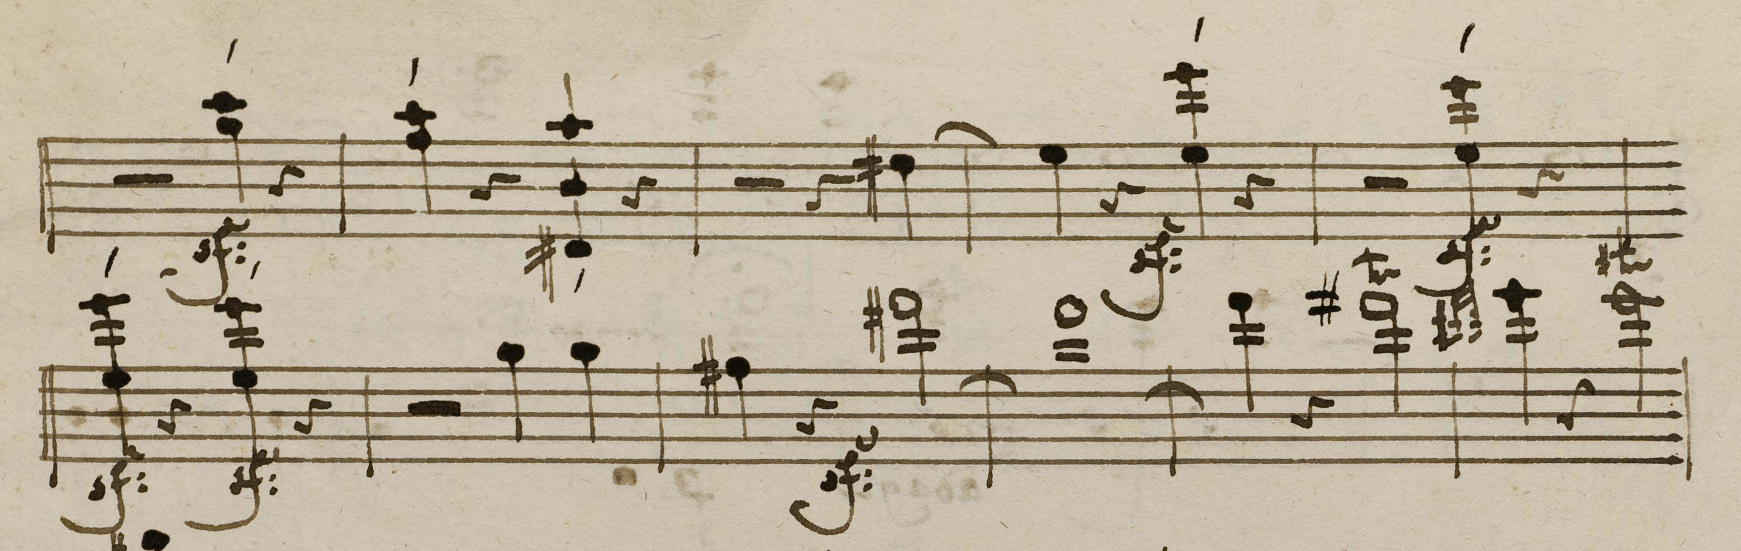
\includegraphics[width=.9\textwidth]{images/chapter1/beethoven_kreuzer_mm66-76.png}}
            \captionsetup{width=.5\textwidth}
            \caption[Mm. 66--76 from Beethoven's \textit{Kreuzer Sonata}. Violin part excerpted from original manuscript.]{Mm. 66--76 from Beethoven's \textit{Kreuzer Sonata}. Violin part excerpted from original manuscript.\footnotemark}
            \label{fig:beethoven}
        \end{figure}
            \footnotetext{\fullcite[]{Beethoven_manuscript}}

    To sum up, two major changes in the printed page have taken place: first, the glyphs which explicitly grant improvisatory latitude to the performer---namely, figured bass indications and the host of baroque ornamentation symbols---have been stripped away, replaced by precise voicings and occasional \textbf{\textit{tr}} markings. Second, beyond the addition of fully-realized harmonies which replace the now-missing figured bass, composers began delineating their idealized performance further still via the use of more frequent and more specific dynamic indications, tempo markings, articulations and expressive text. This is of course not to claim that broader improvisational practices disappeared all together during this period---Beethoven, like the vast majority of his professional peers, was known to have been a talented improviser.\autocite[652--3]{Taruskin_2009b} Further, his explicit instruction in the ``Emperor'' concerto to ``not make a cadenza here, but play immediately the following [...]'' illustrates that performers were still commonly expected to freely improvise at cadences at least as late as 1809---though it gradually became more commonplace over the nineteenth century to merely execute fully-notated composer-provided cadenzas.\autocite[45]{Swain_1988} Thus, perhaps predictably, it seems that the first casualty of the large-scale trend toward the fixity of the sound-concept (which will eventually result in the disappearance of nearly \textit{all} Western art music improvisation by the turn of the twentieth century) is the notation which traditionally represented its \textit{openness}.
    
    Accounts of this decline in performer agency seem, broadly, to take two different tacks; centering either changes in \textit{aesthetic values} over the long eighteenth century or changes in \textit{socioeconomic factors}. Where Charles Rosen cites a ``solid body of aesthetic doctrine which condemned ornament [considered whole] as immoral,''\autocite[1198]{Rosen_1970} Robin Moore's more detailed essay considers aesthetics to be functionally downstream of ``the effect of technological development and industrialization,'' as well as ``the effect[s] of notation and literacy.''\autocite[80]{Moore_1992} Felix Diergarten further expounds on these pedagogical causes by describing an invisible war which took place in nineteenth-century music academies between proponents of the agèd Italian partimento tradition and those of the new German models of music theory.\autocite{Diergarten_2011} Partimento pedagogy held that the most effective means of internalizing realities of musical composition and performance was its practice. Students were exposed early on to countless musical prototypes and exemplars, perhaps the most famous of which was the \textit{regola dell'ottava}---the rule of the octave---which served as a schema by which a student could harmonize arbitrarily complex basslines \textit{ex tempore}. Only via this vocabulary-focused hands-on approach did students gain insight into what motivated particular ``musical moves'' compositionally and, in tandem, learn to build this vocabulary into their personal, improvisatory, network of musical moves. The German approach, on the other hand, eschewed these ``recipes and household remedies'' in favor of logically organized principles: universally applicable rules able to explain in hierarchical terms what motivated movement from tonic to dominant or why some tones seemed to supervene on others\autocite[9]{Diergarten_2011}. Though these two approaches persisted contemporaneously for some time, it was ultimately the latter system which won out---as might be demonstrated by peering at any undergraduate theory syllabus written in the past hundred years or so.

    Robin Moore buttresses this socioeconomic/pedagogical argument and specifically tethers the decline of improvisatory practice to (among many other factors) issues of notation. Per his 1992 paper ``The Decline of Improvisation in Western Art Music'',\footnote{Emphasis in quotes will be mine unless otherwise noted.}

        \begin{smallquote}
            The increasing importance of notation as a pedagogical tool and performance aid in the nineteenth century can similarly be explained in terms of the gradual replacement of the patronage musician at that time with the middle class performer. Scores and written arrangements for the piano were imperative to the dissemination of elite music among a broader audience in two senses. First they allowed for individual family members to learn music themselves, and to avoid the prohibitive costs of hiring professional musicians. [...] Secondly, \textit{notated music provided the detailed performative instructions necessary for those interested in learning to play a style of music with which they were unfamiliar. Sheet music became a means of learning aristocratic music for those who had no exposure to it in its original context.\autocite[72]{Moore_1992}}
        \end{smallquote}

    Here, I think, lies the simple math at the crux of the issue: once a more rarefied ecclesiastical (and/or) scholarly (and/or) aristocratic pursuit, art music had the luxury of a much smaller pedagogue-to-pupil ratio. As such, the tools of its creation and dissemination could be put to much subtler use. Students who had the privilege of close master/apprentice-style tutelage were able to develop literate improvisation schemas which corresponded closely to marks printed on the page. With the explosion of middle class performers (and performance opportunities), musicians had neither the time nor the money to dedicate years to the development of these schemas. Figure~\ref{fig:Corri} illustrates one of the first examples of music published for this growing market ``in »complete« form, with all necessary ornamentation written out in an appropriate manner for those who might otherwise be unable to interpret the score improvisationally."\autocite[72]{Moore_1992} Put simply, new, more ``fixed'' notation conventions (the standard trill in m. 11 and the turn and trill-to-mordant in m. 12) have replaced prior open notations and thereby obviated any knowledge of the delicate art of embellishment.

        \begin{figure}
            \centering
            \fbox{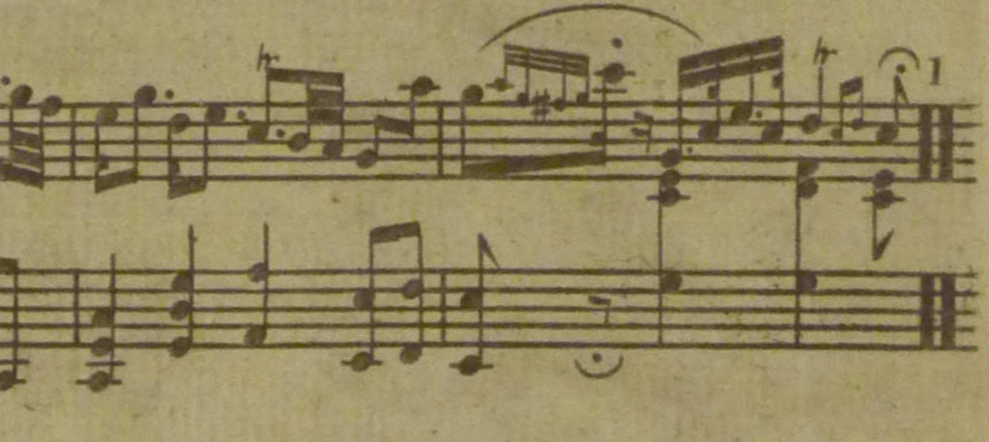
\includegraphics[width=.7\textwidth]{images/chapter1/corri1.png}}
            \captionsetup{width=.5\textwidth}
            \caption[Mm. 11--12 from the first Andante of Domenico Corri's breezy \textit{Loch Erroch Side} Variations demonstrating a carefully-realized cadence---far more ``fixed'' than earlier published keyboard works.]{Mm. 11--12 from the first Andante of Domenico Corri's \textit{Loch Erroch Side} Variations demonstrating a carefully-realized cadence---far more ``fixed'' than earlier published keyboard works.\footnotemark}
            \label{fig:Corri}
        \end{figure}
            \footnotetext{\autocite[]{Corri}}
    
    What was once merely the skeletal framework for a ``finished'' composition necessarily became representative of the entire sonic trace of the work---a condition which was, I take it, inextricable from a concomitant change in taste which demanded that the composer be responsible for the ``entirety'' of the work. Consequently, conservatories and other formal pedagogical centers either willingly or reluctantly began orienting their lessons toward this new fixed model of composition: to oversimplify, it seems that the explanatory power of German theoretical models benefited by having fixed pieces for analysis---complete at time of writing---rather than the more nebulous pre-nineteenth-century works which necessarily varied from performance to performance, relying on performers' input to ever be truly ``finished.''

    By the turn of the twentieth century, this new paradigm of notational fixity was thoroughly entrenched. While pockets of resistance clung tenaciously to life (e.g. in the aforementioned French liturgical tradition), Western art music notation by and large only developed insofar as it fixed the sound-concept of the musical work in finer and finer detail.\footnote{
        Consider, for instance, the growing compass of dynamic indications. Where, for Mozart (1756--91), a range of $\lilyDynamics{pp}$ to $\lilyDynamics{ff}$ was plenty (and these extremes only appear rarely), Tchaikovsky's (1840--93) oeuvre ranged from $\lilyDynamics{pppppp}$ to $\lilyDynamics{ffff}$ in his \textit{Pathétique} and Fifth Symphonies, respectively. Not to be outdone, György Ligeti's (1923--2006) range encompasses $\lilyDynamics{pppppppp}$ (Piano Étude No. 9) to $\lilyDynamics{ffffffffff}$ (\textit{Le Grand Macabre}).
        } 
    To this day, there is a very real sense in which art music in the European tradition is still produced and consumed under the hegemony of this nineteenth-century notation paradigm. To the extent that alternatives exist, they are practiced in the broad historical shadow of western notation---either derived from it (as is the case with the notation commonly used to record and study the Iranian \textit{radif} tradition---if not to teach it) or carved away as a ``subaltern'' which will necessarily be contrasted with it (as is the case with, for example, the various types of Japanese shakuhachi notation). Thanks in no small part to centuries of brutal colonial dominance by a ``global north'' whose modes of musical production often eclipse even long-lived local practices, western notation serves as a \textit{lingua franca} across (not all, but) a broad range of the world's musical styles and practices---both those which might fit under the umbrella of ``art music'' generally, as well as more quotidian vernacular practices. 

    In the next section, I'll discuss in brief the rise of perhaps the most successful challenge to this ``fixed paradigm''---the ascension of notation-mediated jazz improvisation---which coincided with jazz's own ascent from a rather localized vernacular music to a radically transfigured art music all its own. Given that this chapter has thus far served as a gloss of Western art music notation practices, this detour into a discussion of jazz notation might seem tangential. Our ultimate aim here, though, is a cogent analysis of a variety of specific open notation practices in the late twentieth century---many of which sit at the interstices between Western art music and jazz proper. Further, while most would not consider jazz (even in its mature form) to be an offshoot of Western art music \textit{per se}, the two have been, since the latter genre's nascence, hopelessly entwined---sharing mutual creative influence, personnel, theory, technique, and of course notation.
    

    \section[The Afro-diasporic return to open notation]{The Afro-diasporic return to open notation}

    To be crystal-clear up front: Jazz does not bear the same relationship to musical literacy as does western concert music. ``Literacy'' in the sense we have discussed it thus far is simply not a prerequisite for meaningful musical interaction in jazz performance. Paul Berliner's \textit{Thinking in Jazz} (1994), one of the most thorough jazz ethnographies published so far, cites several examples of renowned artists who attained fluency with western notation only quite late in their careers---and indeed stresses that in some cases an over-reliance on printed materials can meaningfully hinder jazz students' development\autocite[111]{Berliner_1994}. We might attribute this to the fact that jazz developed under radically different conditions than did western ``classical'' music. Autodidacticism and musician-to-musician o/aurality (to contrast with the centralized authority of the academy/conservatory and teacher-to-pupil o/aurality) traditionally played a much greater role in jazz than in the European tradition. In instances where students lacked the central knowledge base a formal institution which might favor transmission-by-notation, burgeoning jazz musicians might turn to direct transcription from recordings or other performances to acquire their improvisation schema and library of works. Further, many jazz instructors (despite a full working knowledge of western notation) deliberately de-emphasize(d) reading in their pedagogical practice---instead emphasizing the roles of listening and memory in acquiring and deploying genre-appropriate vocabulary.\autocite[112--3]{Berliner_1994} Debates over the relative worth of orality and literacy in jazz have been hashed out far better than I could hope to achieve here by the likes of Ingrid Monson, Gunther Schuller, and Berliner himself---thus I will stop short of throwing in my two cents on the topic. However, even if we admit to the notion that (as many would perhaps rightly claim) jazz is first and foremost an o/aural tradition, this fact does not preclude our consideration of the pivotal role that notation plays in its (again) pedagogy, acquisition and performance. 

    It is important to note that jazz was ``open'' before it was ever notated. To the extent that jazz performers have adopted techniques of western notation, they have always done so to further the agenda of open, largely improvised performance. That is to say: the primary mode of play in jazz performance centers on highly variegated renditions of existing tunes drawn from any number of creative wellsprings: original compositions, popular songs, folk tunes, etc. How far these renditions depart from some central, organizing artifact (be it one ``ancestral'' recorded performance, one particular arrangement, etc.) also varies from period to period and from sub-genre to sub-genre. While indeed the ``same-but-different'' model adopted by jazz performers bears a strong resemblance to aspects of figured-bass-oriented baroque performance practice, jazz renditions are often strikingly distinct (rhythmically, melodically, harmonically) from their original sources when compared to what we know of Renaissance and baroque improvisation. Figures~\ref{fig:MyFunnyOrig} and~\ref{fig:MyFunnyDavis} illustrate a particularly wide gap between original source and jazz rendition (a gap that forms an important part of Robert Walser's thesis in his fascinating 1993 paper ``Out of Notes'').

        \begin{figure}
            \centering
            \fbox{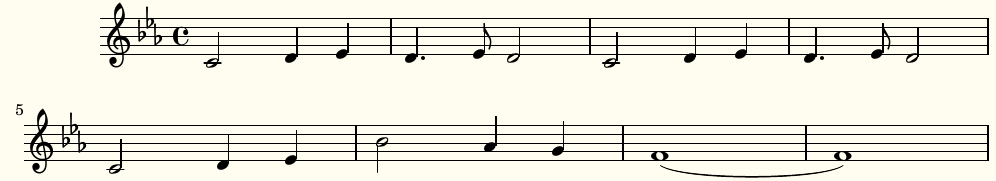
\includegraphics[width=.9\textwidth]{images/chapter1/davis_valentine2.png}}
            \captionsetup{width=.5\textwidth}
            \caption[First eight measures of the chorus to ``My Funny Valentine'' as originally printed in the 1937 edition (virtually identical to countless versions printed in fakebooks since).]{First eight measures of the chorus to ``My Funny Valentine'' as originally printed in the 1937 edition (virtually identical to countless versions printed in fakebooks since).}
            \label{fig:MyFunnyOrig}
        \end{figure}

        \begin{figure}
            \centering
            \fbox{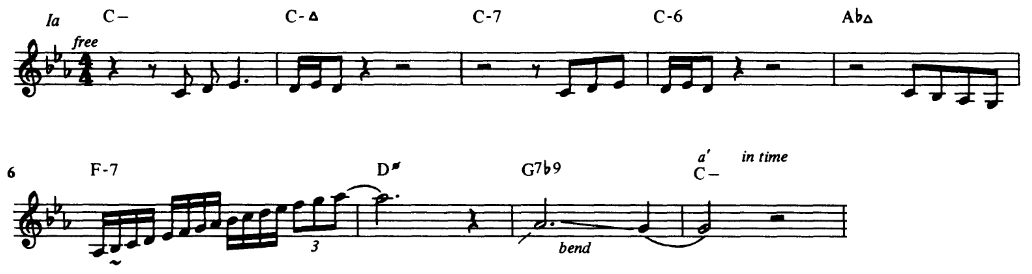
\includegraphics[width=.9\textwidth]{images/chapter1/davis_valentine1.png}}
            \captionsetup{width=.5\textwidth}
            \caption[First nine measures of Miles Davis' melody statement of ``My Funny Valentine," taken from his 1964 recording. As transcribed by Robert Walser]{First nine measures of Miles Davis' melody statement of ``My Funny Valentine," taken from his 1964 recording. As transcribed by Robert Walser.\footnotemark}
            \label{fig:MyFunnyDavis}
        \end{figure}
            \footnotetext{\autocite[]{Walser_1993}.}

    Here, as in the earlier fifteenth-century examples, notation has the ability to ``speak to'' a jazz performer in a particular way, affording a range of potential gestures to be realized in performance. The distinction between Figures~\ref{fig:MyFunnyOrig} and~\ref{fig:MyFunnyDavis}, both (insofar as the language of jazz is concerned) unmistakably instances of the same ``work-concept,'' demonstrates how broad a field of potential is inferred by the symbols on the page. Naturally, these symbols as originally penned were not \textit{deliberately} imbued with these affordances by a composer (``top-down''). Rather, precisely \textit{how} the notation speaks to a performer is contingent on a number of factors---in this example, on Davis' formal training in the western notation paradigm, his experiences with jazz instructors, his countless hours transcribing past performances, his personal taste, etc. While at the time of the cited performance, Davis was undoubtedly ``off book,'' having committed the tune's skeletal framework to memory and no longer requiring printed music in order to faithfully perform his rendition, the $\langle$skeletal framework $\rightarrow$ field of potential$\rangle$ model still obtains. That is to say, a performer unfamiliar with the tune might, when presented with its framework in the form of melody and lead-sheet symbols, arrive at a similarly-structured rendition.


    It is these lead-sheet symbols (e.g. $C^{\Delta}$, $C^{-7\flat5}$, $C^{\circ}$, etc.) which form one of the most salient, concrete points of departure from ``traditional'' (read: nineteenth-century) notation and toward a new, now decidedly Afro-diasporic hybrid model of notation-mediated musicmaking. Mark Abel, in a much-needed 2016 paper on these symbols' history and function traces their origin from their aforementioned ancestral beginnings in figured-bass notation and \textit{alfabeto} (a sixteenth-century derivation of lute tablature) to their formal introduction in the 1920s in popular music charts meant for amateur consumption, then finally to their modern-day use in jazz performance contexts. Per Abel, George Goodwin's ``TuneDex'' cards---bundles of Rolodex-like notecards sold via a mail-in subscription service which featured simplified versions of popular melodies and their attendant chord symbols---were such an overnight success that their sparse notational language became \textit{de rigueur} for jazz and pop musicians across the industry.\autocite[28]{Abel_2016}
    
    These three-part glyphs which indicate an operant chord's root, quality, and extensions (without regard for inversion) were originally employed as labor-saving devices---that is, as a means to obviate any knowledge of tonal harmony on the part of rhythm section players. These were (and still are in pop music compendia) often  accompanied by fingering diagrams for ukulele, guitar, or banjo such that the performer need not possess basic musical literacy in the traditional sense---merely an understanding of the fundamental mechanics of their instrument. However, for Abel, because these chord symbols represent a new layer of abstraction in between the harmony underlying a composition and that harmony's reification in sound, they also afford players a ``radical openness'' in performance, permitting 
    
    %Something weird wrong with the citaton in this paragraph?
        \begin{smallquote}
            new expressive possibilities, and [...] new creative relationships between individuals and collectives capable of eroding the profound schisms between composer and performer, producer and consumer, which have bedevilled the sociology of music in Western modernity.\autocite{Abel_2016}
        \end{smallquote}

    To wit, once chord symbols became part of the standard operating procedure for the composition, dissemination and performance of jazz, he claims, musicians began further conceiving of their improvisations as part and parcel of a harmonic ``grid'' wherein changing chordal fields pertinent to the melody proceed as time progresses. Rather than viewing them as limiting factors which impinge upon improvisatory freedom, Abel sees chord symbols as creative mediators which ``[open up] the rapid `vertical' development of musical harmony,'' facilitating ``alterations and substitutions'' hitherto inconceivable under earlier, more fixed paradigms of harmonic notation. Further, the liberation of the chord progression from a nineteenth-century conception of hierarchical structure \textit{via} these abstract symbols permitted a departure from the notion of a singular key center in both composition and improvisation; paving the way for pieces like the (in)famous middle-period works of John Coltrane (``Giant Steps,'' ``Countdown,'' et al.) which flit liberally from temporary tonic to temporary tonic.
    
    In ``Radical Openness,'' Abel stops short of drawing any particular musico-ethnographic conclusions regarding the widespread adoption of the lead-sheet symbol in jazz performance. At the risk of verging into hermeneutics, I would put forward that perhaps we ought to interpret the rise of the lead-sheet---arguably the most important integration of art music and open notation since the decline of figured bass---not solely as a happy accident stemming from the decline of musical literacy in the early twentieth century, but also as an \textit{active assimilation} of old-guard Eurocentric musical knowledge by a growing pool of artists working in a relatively young Afrocentric paradigm. In essence, the lead-sheet served as a new musical technology developed via a fusion of the now ``fully-fixed'' European art music notation and the mediated openness of Afro-diasporic o/aural practices. That such a fusion could be catalyzed by such a ``low-brow,'' utilitarian notational device as the chord symbol rather than, say, by a concerted effort on the part of some great musical innovator should not go without mention.

    Each chord symbol (as employed by the jazz improviser) serves as a sort of map of a particular harmonic territory; one which applies to the melody of a tune (insofar as it, like a figured bass symbol, indicates which sort of harmony ought to be played underneath the recited melodic line) as well as, canonically, to the harmonic structure of the improvisation which follows. As they progress, each glyph ``projects'' a particular field of potential musical action into the mind of the performer. As with the other open notation schemes we have observed thus far, players are then able to make informed musical moves via a combination of pre-performance data (musical upbringing, personal taste, spoken instructions) as well as the creative constraints on the page. 

    As such, I take it that this experience does not fundamentally differ from the phenomenology of the figured-bass interpreter and thus does not represent some profound new modulation of the performer/composer relationship (as perhaps the genres' very different sonic traces would imply). However, lead-sheet interpretation is particularly interesting in that it represents an instance of ``parallel evolution'' (albeit one displaced by a few hundred years) with the aforementioned figured bass (and/or \textit{alfabeto}, etc.) insofar as it rose to prominence as a musical technology out of a similar necessity: the need to disseminate and perform vast quantities of new music by equally new, less literate sectors of the musical public as well as the need to save material and labor on copying and music publishing. The lead-sheet differs, however, in that, per Abel's claims, it was able to exceed its humble origins and form a key part of the corpus of the new American art music \textit{non plus ultra}, ultimately facilitating a new sort of harmonic conception of musical forms and thereby paving the way for the myriad harmonic languages with which jazz musicians express themselves through to the present day.

    Given the rapid adoption and prevalence of this new musical technology by the end of the second world war, one might expect to see its use somehow reflected in the score-making practices of more traditional art-music composers. Ultimately, though, while jazz (in several understandings of the term) would absolutely have an outsize impact on the new ``classical'' music of the mid-twentieth-century, jazz's lead-sheet model of open composition would never be imported wholesale. However, the 1950s and 1960s \textit{did} bring with them a veritable explosion of innovative and highly individualistic new modes of composition which in turn required attendant new forms of notation. In this chapter's final section, I will examine what I take to be the most historically impactful of these, including, crucially, the extent to which they were (or indeed were not) expressly tied to jazz's ethos, structure, and notational reforms.

   
    %\begin{notestuff}
    %\begin{enumerate}
        %\item Jazz was open before it was notated. Therefore to the extent that it uses notation, it uses OPEN notation. As we saw our c.s.l. and figured bass examples, scores in jazz performance represent ``unfinished'' skeletal frameworks which, if performed, would represent particularly impoverished renditions of the works they represent.

        %\item These frameworks tend to be perhaps more open still than were earlier figured bass structures and tunes may be ``stretched'' often to incredible lengths while still retaining their core identity as an instance of a particular musical work. {Walser Miles Davis excerpt here.}

        %\item What's the wrap-up here? Make a claim about this rebirth of openness impacting avant-notation. Or at least claim that it's hard to make claims.
        
   %     \end{enumerate}
   % \end{notestuff}
    
    \section[Postwar: new open musics]{Postwar: new open musics}

    As I hope has been demonstrated by this point, the histories of our numerous literate art musics are replete with examples of notation having been modified or invented wholesale to suit some material need in the composition, distribution, learning, and performance of musical works. Indeed, the concert music of the mid-twentieth century was no exception. To the contrary, new forms of open music taken together formed a crucial ``reaction formation'' (if you'll permit the analogy) against the rising tide of serialist compositional practices which by that time were \textit{de rigueur}; serving as the received language of European-style avant-gardism.\autocite[14--5]{Taruskin_2009d}

    This is of course not to claim that this new interest in musical openness was entirely coextensive with a new fervor for creative notations. Many noteworthy pieces were constructed which eschewed the romantic fixity of sound-concept using little more than traditional notation---albeit occasionally modified to better suit its new purpose. Before it was amended and republished, Luciano Berio's original \textit{Sequenza} (1958) (excerpted in Fig.~\ref{fig:sequenza}) experimented with flexible ``proportional'' rhythmic notation\footnote{Paul Griffiths identifies this as `space-time notation,' though I've not heard the term elsewhere.} and Terry Riley's standout \textit{In C} (1964) (Fig.~\ref{fig:inc}) permits performances which widely vary in personnel, duration, etc. by employing short modular units of traditional notation to be repeated \textit{ad libitum} by individual performers.

         \begin{figure}
            \centering
            \fbox{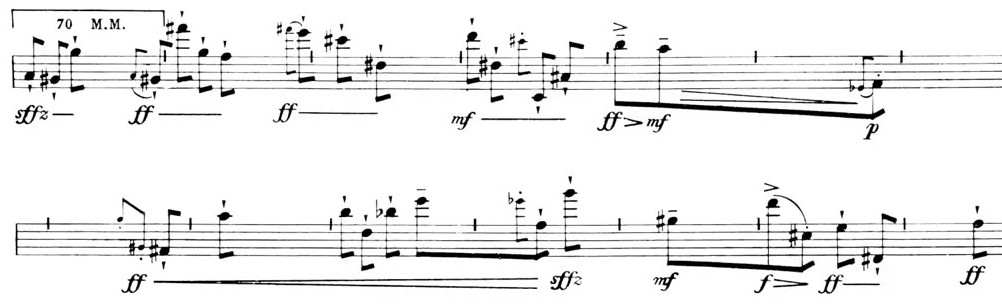
\includegraphics[width=.9\textwidth]{images/chapter1/sequenza1crop.jpg}}
            \captionsetup{width=.5\textwidth}
            \caption[First two systems from the original edition of Luciano Berio's \textit{Sequenza} (I, 1958) which deploys quasi-open proportional notation.]{First two systems from the original edition of Luciano Berio's \textit{Sequenza} (I) which deploys quasi-open proportional notation.\footnotemark}
            \label{fig:sequenza}
        \end{figure}
            \footnotetext{\autocite{Berio_1958}}

            \begin{figure}
            \centering
            \fbox{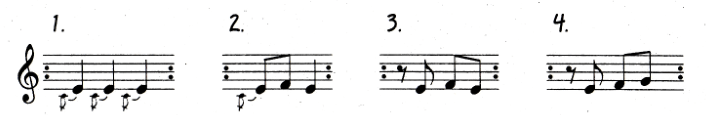
\includegraphics[width=.9\textwidth]{images/chapter1/inc1.png}}
            \captionsetup{width=.5\textwidth}
            \caption[First four modules from Terry Riley's \textit{In C} (1964).]{First four modules from Terry Riley's \textit{In C} (1964). An open score featuring pared-down traditional notation.\footnotemark}
            \label{fig:inc}
        \end{figure}
            \footnotetext{\autocite{Carl_2010}}

    However, insofar as they represent \textit{such} a drastic departure from traditional methods of musical representation, it is often the pieces employing ``neo-notation'' (i.e. any built-to-purpose notation which distinguishes itself from canonical common-practice methods, be it in service of ``open music'' or not) which most captivate composers, musicians, and laity alike. Most authoritative sources point to the earliest days of the 1950s as the beginning of this new compositional mode; specifically citing ``New York School'' composer Morton Feldman as the first to work in this style. Even John Cage, perhaps the best-known composer of open music in this vein, credits Feldman with the style's genesis (though he dubbed it ``[music] indeterminate with respect to its performance'').\autocite{Dohoney_2017} The first system of \textit{Projection 1} (1950), the composition credited with launching this new fervor for open works, is shown in Figure~\ref{fig:feldman1}.

        \begin{figure}
            \centering
            \fbox{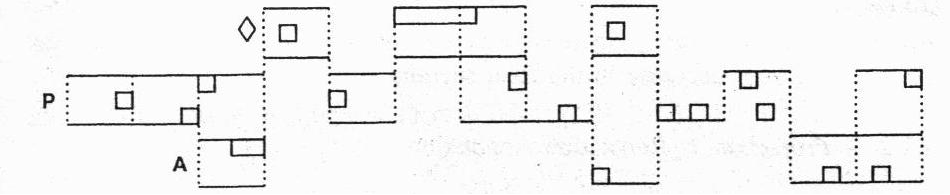
\includegraphics[width=.9\textwidth]{images/chapter1/projection1crop.png}}
            \captionsetup{width=.5\textwidth}
            \caption[First system of Feldman's \textit{Projection 1} for solo `cello (1950). Often cited as the first noteworthy instance of ``graphic'' neo-notation.]{First system of Feldman's \textit{Projection 1} for solo `cello (1950). Often cited as the first noteworthy instance of ``graphic'' neo-notation.\footnotemark}
            \label{fig:feldman1}
        \end{figure}
            \footnotetext{\autocite{Feldman_2002}}

    Though the graphic system he employs seems quite opaque at first blush, Feldman is quite explicit with how his notation is to be interpreted, providing a block of text right at the top of the page:

        \begin{smallquote}
            \textsc{Timbre is indicated: $\diamond$ = harmonic; P = pizzicato; A = arco. Relative pitch (high, middle, low) is indicated: $\overline{\rule{1.2ex}{1.2ex}}$ = high; $\overline{\underline{\rule{1.2ex}{1.2ex}}}$ = middle; $\underline{\rule{1.2ex}{1.2ex}}$ = low. Any tone within the ranges indicated may be sounded. The limits of these ranges may be freely chosen by the player. Duration is indicated by the amount of space taken up by the square or rectangle, each box (\myline[dashed]  \myline[dashed]) being potentially 4 icti. The single ictus or pulse is at the tempo 72 or thereabouts.\autocite{Feldman_2002}}
        \end{smallquote}

    Here, Feldman cedes absolute control over some traditionally fixed musical parameters (pitch, duration) while maintaining control of others (timbre, instrumentation, order of events). The radical break from tradition posed by the ``graphics'' used to represent these events belies the fact that the work is only slightly ``further open'' than many earlier, more conventionally-notated works (e.g. similarly ``proportional'' seventeenth-century unmeasured preludes of the form shown in Figure~\ref{fig:nonmesure}). Only with regard to the pitch axis is Feldman's work truly phenomenologically distinct from these earlier works: a performer must now creatively decide (a) (pre-performance) what range to assign to the upper/lower bounds of each box and (b) (in-the-moment) precisely which pitch in that range to execute during each event.

    Feldman would continue, over the next few years, to develop his ``graph'' compositions alongside his more traditional works, including forays into pieces for larger ensembles like \textit{Intersection 1} (excerpted in Figure~\ref{fig:feldman2}) which grants an additional axis of autonomy to performers by giving them the opportunity to place their attacks at any point in the time segments demarcated with dotted verticals.

        \begin{figure}
            \centering
            \fbox{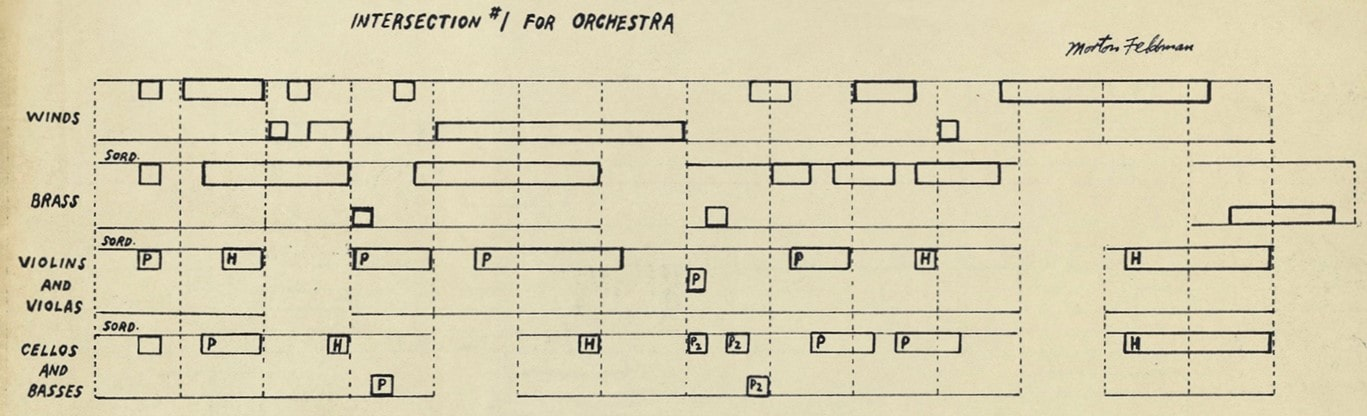
\includegraphics[width=\textwidth]{images/chapter1/feldmanintersectioncrop.jpeg}}
            \captionsetup{width=.5\textwidth}
            \caption[First system of Feldman's \textit{Intersection 1} for full orchestra (1951). Another early ``graphic'' work.]{First system of Feldman's \textit{Intersection 1} for full orchestra (1951). Another early ``graphic'' work.\footnotemark}
            \label{fig:feldman2}
        \end{figure}
            \footnotetext{From a 1962 publication cited in \autocite{Dohoney_2017}}

    Of course, Feldman did not conceive of this new means of representation in a vacuum. His New York School peers John Cage, Earle Brown, Christian Wolff, and associate performer/composer David Tudor similarly sought musical indeterminacy via ``graphic'' notations during this period. However, despite the fact that these composers are frequently cited in the same breath (of which I, too, am now guilty), their motivations for and implementations of neo-notation sometimes differed greatly. Of primary note is Earle Brown's \textit{Folio}, a set of seven pieces penned shortly after Feldman's series of works and published in 1953 which took a remarkably different tack.\footnote{\textit{Folio} is now most often referenced as \textit{Folio and 4 Systems} thanks to a more recent publication which tacks the latter piece to the end of the collection.} Brown, formally trained for many years as a jazz musician, was perhaps more eager (or at least less reluctant) to, with the help of a more active interpreter, co-author his compositional efforts.\autocite{Ryan_2002} As such we find in \textit{Folio} a variety of new symbolic structures which vary in their familial resemblance to traditional notation. Figure~\ref{fig:brownfolio} provides excerpts of the first three pieces from this series, \textit{October 1952}, \textit{November 1952}, and quite possibly the most-reproduced ``graphic'' score extant, \textit{December 1952}.

    %\footnote{I will continue to self-consciously place the term ``graphic'' notation in scare quotes as the word is far too vague to be deployed as often as it is in relevant literature. It's commonly used to refer to techniques as disparate as Xenakis' very precise percussion scores (which feature only very little creative latitude), Cardew's \textit{Treatise} (which is in essence entirely a work of graphic art which only incidentally produces music), Ligeti's \textit{ex post facto} ``listening score'' for \textit{Artikulation} (never meant to be used for performance, only perusal), and Xenakis' pre-compositional material for \textit{Metastasis} (not a score at all). I much prefer, whenever possible, to use more precise language to disambiguate these very different uses for ``graphics'' in the context of music representation.}

        \begin{figure}
            \centering
            \fbox{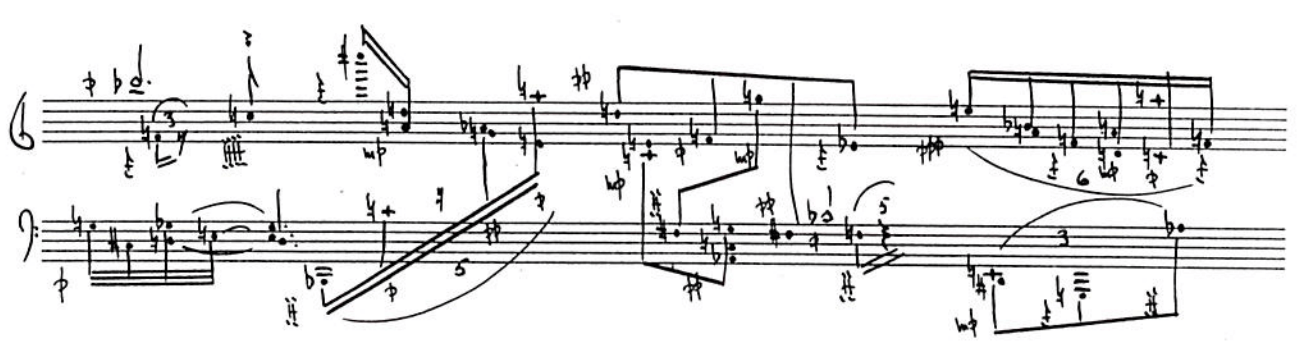
\includegraphics[width=.7\textwidth]{images/chapter1/oct52.png}}

            \vspace{5pt}
            
            \fbox{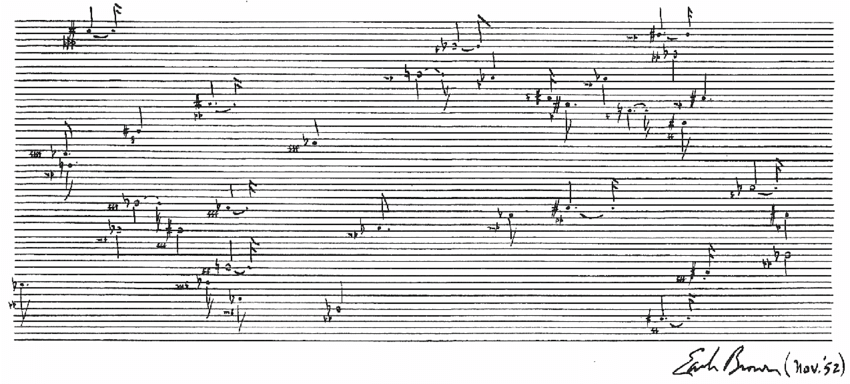
\includegraphics[width=.7\textwidth]{images/chapter1/nov1952.png}}

            \vspace{5pt}
            
            \fbox{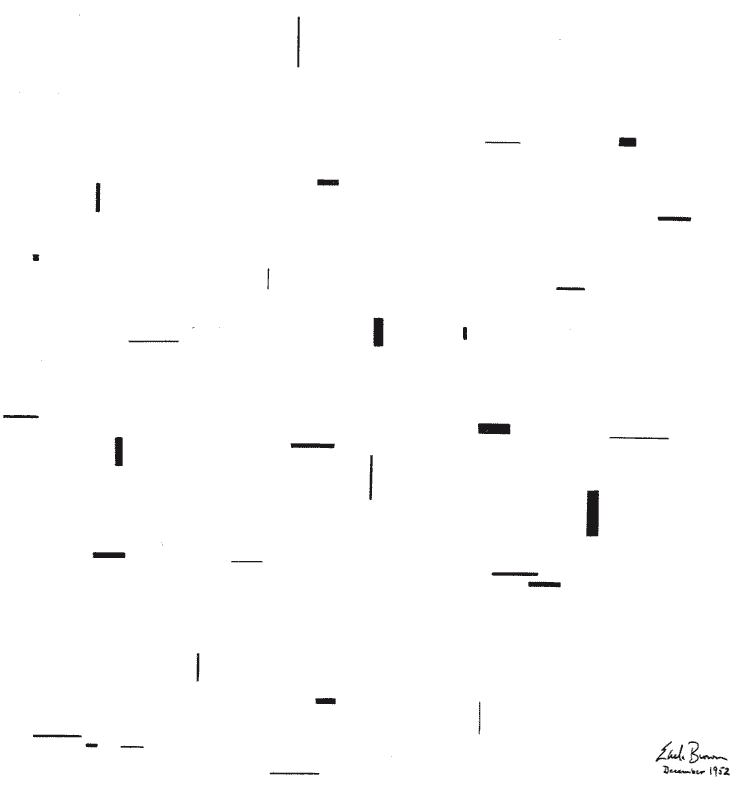
\includegraphics[width=.5\textwidth]{images/chapter1/dec52.png}}
            \captionsetup{width=.5\textwidth}
            \caption[Excerpts from Earle Brown's \textit{Folio} (1953). From top to bottom: First system from \textit{October 1952}; Entirety of \textit{November 1952}; Entirety of \textit{December 1952}.]{Excerpts  from Earle Brown's \textit{Folio} (1953). From top to bottom: First system from \textit{October 1952}; Entirety of \textit{November 1952}; Entirety of \textit{December 1952}.\footnotemark}
            \label{fig:brownfolio}
        \end{figure}
            \footnotetext{\autocite[2--8]{Brown_1986}}

    That scores of this heterogeneity were composed within mere months of each other and published as one package speaks, perhaps, to the sense of newness and experimentalism that led to their creation. \textit{October} (for piano), despite its somewhat whimsical engraving and lack of barlines, was given a standard metronome marking of $\crotchet$ = 135 and was intended to be performed ``straight-ahead.'' \textit{November} (marked ``for piano(s) and/or other instruments or sound-producing media'' and given the alternate title ``Synergy'') maintains at least a tenuous relationship to traditional notation in that it still employs traditional dot/stem/flag notation with accompanying dynamic markings. However, the instructions provided with the score give an entirely different perspective:

    \begin{smallquote}
    The frequency range will be relative to that of each instrument performing the work. \textit{To be performed in any direction from any point in the defined space for any length of time}. Tempo:\textit{ as fast as possible to as slow as possible [...] inclusive}. Attacks may be interpreted as completely separated by infinite space, collectively in blocks of any shape, or defined exactly within that space. Lines and spaces may be thought of as tracks moving in either direction (horizontally at different and variable speeds) and clef signs may be considered as floating (vertically over the defined space) [...]\textit{ The defined space may be thought of as real or illusory, as a whole or in parts}.\autocite[1]{Brown_1986}
    \end{smallquote}

    Like Feldman, Brown permits the vertical compass of the ``graphic'' to map to the range of the performer's instrument. Unlike Feldman, though, who only \textit{further abstracted} the representation of musical events in time, Brown here has shattered one of the most fundamental principles of western music notation which had held steadfast since at least the era of Guido d'Arezzo: the mapping of time to the \textit{x}-axis. Play no longer proceeds \textit{top left} $\rightarrow$ \textit{bottom right} but rather ``proceeds'' in a manner entirely up to the performer's discretion. What information Brown's bespoke notation actually \textit{provides} a performer, then, is actually rather vague. Horizontal lines which typically demarcate precise pitch quanta have become indefinite signifiers of ``vertical'' distance. The notes' forms (shape, stems, flags) have, in light of his careful instructions, become virtually empty of concrete meaning. We might assume that, insofar as they remain unmentioned in the notes, dynamic markings are meant to be observed ``as written''---in which case they would serve as the sole fixed parameter in the piece save the number of attacks. Even without consulting firsthand accounts of the piece's creation; taking this evidence together it becomes clear that Brown has begun centering the ``visuality'' (or ``aesthetic,'' if you like) of his glyphs over and above any denotative symbolic value they might otherwise provide. In a crucial inversion, this visuality now drives the sound-concept and the production of sound---completely contrary to the traditional state of affairs where a composer chooses symbols for their denotative content in order to bring about a desired sound-concept.\footnote{
        Certainly, a number of earlier examples could be said demonstrate a sort of privileging of notation's aesthetic in composition---most notably minor composer Baude Cordier's ``Belle, bonne, sage'' which renders a fifteenth-century chanson in the shape of a heart. Even Telemann, in his \textit{Gulliver Suite} experimented with ``eye music'' which similarly wrapped conventional sonic products in a visually arresting package. These, while of limited historical interest, do not, to my mind, prefigure the explosion of new ``visual composition'' in mid-twentieth century.
        }
    This new orientation toward the visual promptly reaches its apotheosis in \textit{Folio}'s third piece: \textit{December 1952}---by far Brown's most well-known work. Having been inspired by Alexander Calder's ``mobile'' sculptures which bear no one consistent visual trace, Brown writes (emphasis his):

    \begin{smallquote}
         The performer was asked to consider these [graphic] elements in this manner only at the moment---and they could be changed continually [...] So, \textit{December 1952} was generated from that very early concern with trying to create something which was a \textit{score} comparable to a visual mobile.\autocite{Brown_2008}
    \end{smallquote}

    While it is often spuriously claimed that \textit{December} was proffered entirely without performance directions in a sort of Dadaist flourish (frequently by authors who ought to know better), in fact at the time of its 1953 publication its instructions reproduced in full read thus:\footnote{Inexplicably, Paul Griffiths makes the claim that of indeterminate scores, \textit{December 1952} was ``at once the earliest, the most enigmatic (there being no instructions about how these shapes are to be realized as sound)'' found in \autocite{Griffiths_2011}}

        \begin{smallquote}
            The composition may be performed in any direction from any point in the defined space for any length of time and may be performed from any of the four rotational positions in any sequence. In a performance utilizing only three dimensions as active (vertical, horizontal, and time), the thickness of the event indicates the relative intensity and/or (where applicable instrumentally) clusters. Where all four dimensions are active, the relative thickness and length of events are functions of their conceptual position on a plane perpendicular to the vertical and horizontal planes of the score. In the latter case all of the characteristics of sound and their relationships to each other are subject to continual transformation and modification. \textit{It is primarily intended that performances be made directly from this graphic ``implication'' (one for each performer) and that no further preliminary defining of the events, other than an agreement as to total performance time, take place.} Further defining of the events is not prohibited however, provided that the imposed determinate-system is implicit in the score and in these notes.\autocite[1]{Brown_1986}
        \end{smallquote}

    Here Brown helpfully provides for two distinct modes of play. The first (in my experience the most frequently adopted method) retains the overall strategy described in \textit{November}, only with the piece's glyphs abstracted one degree further from traditional notation; indicating duration with horizontal extension and dynamic with stroke thickness rather than a \textbf{\textit{pp}}/\textbf{\textit{ff}}-style glyph. The second, perhaps more opaque option has the performer imagine a virtual plane extending from the page. What appear to be two-dimensional rectangles are actually projections of three dimensional objects at various distances from the viewer along this \textit{z}-axis. In either case, Brown makes clear that no preconceived direction-of-play is meant to obtain and that the page may be rotated in any of the four cardinal orientations pre-performance. 
    
    We should note that where earlier improvisation-oriented scores left the precise boundaries of their openness (i.e. the breadth and depth of notation's fields of potential) up to the training and good taste of their performers, Brown (and to a lesser extent Feldman) take great pains to reify these boundaries in prose to be considered prior to performance. By explicitly granting performers the opportunity to choose between multiple interpretive schemes, Brown forges a new sort of relationship between composer, performer and score---one conveyed not through traditional pedagogical/experiential channels but one defined \textit{in situ} by the composer himself.
    
    I have taken, perhaps, a disproportionate amount of time to discuss these early neo-notational works (despite the fact that Feldman quickly abandoned these ``graphic'' forays in favor of a return to traditional work which only \textit{felt} improvisatory) for one important reason: By way of these first forays, these two composers, Feldman and Brown, have articulated (albeit imperfectly) the primary paradigmatic rupture between two classes of open ``graphic'' scores which persists in some form to the present day. We might sum up this coarse division in the following tree diagram (Fig.~\ref{fig:soundvimage}):

        \begin{figure}
            \singlespacing
            \centering
            \begin{forest}
                forked edges,
                for tree={parent anchor=south, child anchor=north,draw,align=center,edge={-latex}}
                [\textsc{new compositional}\\\textsc{openness/``indeterminacy''}
                 [traditional\\notation
                    [{ex: \textbf{\textit{In C}}\\(1964)},tier=word]
                    ]
                 [neo-notation
                  [``sound-first''\\neo-notation
                    [{ex: \textbf{\textit{Projection I}}\\(1950)},tier=word]
                    ]
                  [``image-first''\\neo-notation
                    [{ex: \textbf{\textit{December 1952}}\\(1952)}, tier=word]
                    ]
                 ]
                ]
                \end{forest}
            \captionsetup{width=.5\textwidth}
            \caption{One articulation of notation paradigms during the ascendance of new open musics in the mid-twentieth century.}
            \label{fig:soundvimage}
        \end{figure}

    Works which seek to explore new (or indeed return to old) open forms fall into two broad categories: those which modify (often by paring down) traditional notation and those which introduce new notations for the purpose. Though there is certainly more nuance to be found than is represented here, this latter group tends to divide into two ideologically distinct further categories: Scores which begin from sound- (or process-) concepts which hope to attain an imagined sound world or creative procedure via a novel method of encoding (i.e. ``sound-first'') and those which hope to elevate some visual object (e.g. \textit{December 1952}'s line-segment array) to the status of a \textit{sounding} object; posing it to the performer(s) as an open question of interpretation (i.e. ``image-first'').\footnote{Of course, this could never be a hard-and-fast boundary. There is no reason to imagine that Feldman wasn't to some degree motivated by the sheer novelty and appearance of his new symbolic language or that Brown did not hear an abstract \textit{klangwelt} in his head which motivated \textit{December}. Based, though, on Brown's repeated appeal to visual inspiration and metaphor, I think this is a reasonably safe, if blunt, assessment.} 

    These two approaches are drawn into even more stark contrast when one considers their underlying motivations. It is telling that by 1954, Feldman had entirely abandoned his prolonged experiment with graph (his term) scores, evidently on grounds that they ``liberat[ed] the performer'' to too great a degree. While his scores achieved their initial goal of allowing for an unpredictable, non-replicating sonic trace which did not rely on his particular tastes, habits, and conditioning, Feldman was clearly dissatisfied with the extent to which his performers' creative autonomy crept into the works.\autocite[99]{Taruskin_2009d} Despite an errant indication in his graph score \textit{Marginal Intersection} (1951) for a player to perform a line ``as in a jazz ensemble,'' Feldman clearly did not share in the ethos of jazz musicians who, too, deployed novel notation mechanisms in order to promote a new form of open music.\autocite{Dohoney_2017}

    This jazz-avoidant (occasionally jazz-hostile) orientation among America's hypermodern art-music composers forms one of the primary motivations behind George Lewis' much-cited paper ``Improvised Music after 1950: Afrological and Eurological Perspectives'' and certainly extends to John Cage who, even more frankly than Feldman, denounced the creative processes underlying jazz improvisation, distancing his own ``indeterminate'' works from it whenever possible. Lewis hypothesizes that despite this consistent denunciation, the performance practices which emerged during this period of New York School flourishing are inextricably bound up in the radical musical advances made by America's \textit{other} modernist school of composition: jazz (bebop in particular---not coincidentally also ``headquartered'' in New York City during the 1950s). Lewis sees this reluctance to own up to the clear parallels between these two open musics as essentially rooted in a creeping form of anti-Black racism which tainted the artistic efforts of Black Americans as ineluctably low-brow, unserious, or backward-facing.\autocite{Lewis_2002} 

    To be sure, not to say every New York School associate was equally dismissive of the Afrological avant-garde. Earle Brown himself, a professional jazz trumpeter prior to his turn toward concert music, speaks candidly of the extent to which jazz performance practice motivated the form and content of his open works. From a 1991 interview:

        \begin{smallquote}
            \begin{itemize}
                \item \textbf{BD (Bruce Duffie):} Was the notation your own, or was the notation borrowed from other people that discovered it first?
                \item \textbf{EB (Earle Brown):} No, it was completely my own. I first started doing these things in 1951 and '52, and what occurred to me, from a jazz background, was the freedom and the flexibility that jazz has from performance to performance.
                \item \textbf{BD:} Yes. They're never the same. They're improvisatory.
                \item \textbf{EB:} They're never the same twice. But if you play \textit{How High the Moon} seventeen times, you know that it's \textit{How High the Moon}, even though it's never, in detail, the same twice. That excited me.

                \centering
                    \noindent\rule{2cm}{0.4pt}
                    
                \justifying
                \item \textbf{EB:} [...] But what occurred to me as an ex-jazz musician was why can't the variations be a function of the interaction of the musicians with the material that I have composed? One of the greatest things about jazz is the instant, instantaneous communication.  One played [sings a line] and then the other one goes [sings an answering line].  It’s like you and I having a conversation where we exchange ideas.  That’s always one of the most beautiful things to me about jazz.  So that’s what I tried to introduce, and this goes all the way back to your first question — why new notation, and why the scores look different than other people’s scores.  It’s because I want to introduce the possibility of the musicians not only playing what I write, but interacting like a human family of friendly people.\autocite{Duffie}
            \end{itemize}
        \end{smallquote}

%    \begin{notestuff}
%        Amend this statement to put it more in line with M's reading of Lewis.
%    \end{notestuff}

    \noindent Here, Brown highlights that crucial aspect of jazz performance cited in the previous section: the seemingly infinite malleability of its work-concepts. Given that Brown undoubtedly experienced this malleability via the same notation mechanisms jazz players employ today (i.e. via open melodies and chord symbols), I think it is no great logical leap to suggest that this ``Afro-diasporic return'' to open forms significantly impacted his decision to ground his music in a new notation. While Brown's frankness with regard to this line of influence appears to be the exception rather than the rule, it nevertheless serves to illustrate productive cross-talk between these two musical paradigms---an important byproduct of which were the notation schemes at the heart of this research.


\section{Conclusion}

    With greater and greater intermingling of (``classical,'' ``jazz'', ``free improvisation'') art music spheres in the twenty-first century, more open scores are being composed today than ever were during the 1950s and '60s. The large-scale ``democratization'' of the avant-garde thanks to art's newfound accessibility on the internet has led, I think, to a measure of mainstream acceptance of the viability of the open score as part of the art music landscape. Even ``mainstream'' institutions now occasionally admit these radically open works into their repertoire (albeit usually those by the now-venerated New York School composers themselves). Given that we are at a local apex of the production and consumption of notation-mediated open music, and given that the variety of o/aural-literate traditions underpinning the creation of these works is now more diverse than ever, the comparative lack of rigorous analysis and critique of these fascinating works is somewhat startling. When discussions of notation-mediated open music \textit{do} appear (either in lay-facing publications or in ``the literature''), authors often demonstrate a lack of interest in investigating precisely what sets one open work apart from the rest. 

    That is to say: despite the fact that ``graphic score'' and ``graphic notation'' are common terms of art familiar to anyone who has completed a college-level music history sequence, these terms are wholly inadequate to describe the broad swath of notation-mediated open musical works. I take it that there is an important difference-in-kind between these ``image-first'' (by far the most prevalent and most-discussed form of open ``graphic'' scores) and the often more intellectually knotty but lesser-appreciated ``sound-first'' open works. These two broad categories display radically distinct initial motivations, construction methods, performance phenomenologies, and attendant structures of performer/composer agency. There have been very few concerted attempts to elucidate these differences, to categorize works \textit{according} to these aspects, to taxonomize the varieties of open musical work, or to highlight trans-historical parallels between these and other musics.

    The following chapter will take on the much-needed task of (a) describing in more detail the varieties of notation-mediated open music in terms of these motivations, methods, structures of agency, etc., specifically focusing on these under-discussed ``sound-first'' composition techniques and (b) addressing the few incisive scholarly efforts which lay the foundations for a greater understanding of these works.


% \begin{notestuff}
%     \begin{itemize}
% %\item worth mention that the feldmanian approach is directly tied to a fundamental mistrust of performer agency, given that in 1954 Feldman would abandon his new notation on ground that it ``liberat[ed] the performer'' to too great a degree. This betrays a fundamental sort of ideological opposition to the basic experiences of jazz performance practice---one famously shared by Cage.

% %On the other hand, the Brownian model was developed by a jazz musician who seemed much less reluctant to admit the biases, habits, tastes of his performers into the body of his own works. This seems noteworthy

% %\item writers callously lump these things together, but it's critical to a more thorough understanding of how notation mediates performance to really pull these apart! in the next chapter i'll blah blah

% \item discussion of the mistrust of ``improv'' in denotative graphic scores like Feldman's sets up the uniqueness of somebody like Braxton who does use denotative notations but does so in service of improv rather than despite it.
%     \end{itemize}
% \end{notestuff}

% FOR DISCUSSION OF NOV + DEC and FELDMAN's instructions
%\begin{notestuff}
    %\begin{itemize}
    %\item I'm spending so much time on these earliest scores because they stand in for the fundamental schism in neonotations that I'm getting into in ch. 2 and they form the model for essentially all notational-exploratory works which follow in coming decades.

    %\item By all accounts feldman's works sought a particular sound-world
    
    %\item Brown's approach was visual first, per his citing Calder
    
    %\item if one thing sums up this era of notational practice, it's that now musics are being composed which place notation in the driver's seat -- experiments with the VISUAL are changing our attendant SOUND WORLDS rather than the reverse (what accounts for this?)

    %\item This explosion is of course intimately tied up with (though not coextensive with) a parallel new interest in open musics of all flavors (indeterminacy, improvisation, aleatory)

    %\item Obviously fascination with the visual and a linking between visual and aural creativity are not a new phenomenon -- historical examples do exist which ``privilege'' the visual. However nothing compares to the visual experimentalism that characterized the mid-century.

    %\item Accounts of the motivations behind these innovations differ drastically. Firsthand accounts by often fairly forthright composers point to a number of influences. A certain intellectual tradition argues that this new open music craze is \textit{essentially} downstream of Afrocentric improvised music traditions --- while I think there's real merit to these arguments and a hermeneutic sense in which they hold water, I think the real story is more complicated  

    %\item in fact there are SO many new methods of notation that we begin to suffer from a lack of vocabulary with which to differentiate them. they tend to all get lumped in under the category ``graphic notation,'' which is too broad a category to be of any use.                                                                                 
    %\end{itemize}
%\end{notestuff}

%%%%%%%%%%%%%%%
% END COPY %%%$
%%%%%%%%%%%%%%%
